%%%%%%%%%%%%%%%%%%%%%%%%%%%%%%%%%%%%%%%%%%%%%%%%%%%%%%%%%%%%%%%%%%%%%%
% Lớp 11 | Hàm số lượng giác và phương trình lượng giác | Hàm số lượng giác và đồ thị
% Dạng 1D1?4-4: Xét tính chẵn, lẻ
% Số câu: 90  (sinh tự động bởi tach_cau.py; từ nay thầy sửa trực tiếp file này)
%%%%%%%%%%%%%%%%%%%%%%%%%%%%%%%%%%%%%%%%%%%%%%%%%%%%%%%%%%%%%%%%%%%%%%

%%%%%%%%%%%%%%%% TRẮC NGHIỆM 4 PHƯƠNG ÁN %%%%%%%%%%%%%%%%

% nguồn: Ok_Toan11_TracNghiem_Lan2
\begin{ex}%[1D1N4-4]%[ma:e096794c]
	Mệnh đề nào dưới  đây đúng?
	 \choice
		{Hàm số  $y=\cot x$ là hàm số chẵn}
		{Hàm số $y=\sin x$ là hàm số chẵn} 
		{Hàm số $y=\tan x$ là hàm  số chẵn}
		{\True Hàm số  $y=\cos x$ là hàm số chẵn}
	 \loigiai{
		Xét hàm số $y=\cos x$ có tập xác định $\mathscr{D}=\mathbb{R}$.\\ 
		Với mọi $x\in \mathscr{D}\Leftrightarrow-x\in \mathscr{D}$ và $\cos  x=\cos \left(-x\right)$.\\ Do đó hàm số $y=\cos x$ là hàm số chẵn.
	} 
\end{ex}

% nguồn: Ok_Toan11_TracNghiem_Lan2
\begin{ex}%[1D1N4-4]%[ma:a3f442ef]
	Trong các khẳng định sau đây, khẳng định nào đúng? 
	 \choice
		{Hàm  số $y=\sin x$ là hàm số chẵn}
		{Hàm số $y=\cos x$ là hàm số lẻ} 
		{\True Hàm số $y=\tan x$  là hàm số lẻ}
		{Hàm số $y=\cot  x$ là hàm số chẵn}
	\loigiai{ 
		Xét  hàm số $y=\tan x$ có tập xác định $\mathscr{D}=\mathbb{R}\setminus\left\lbrace \dfrac{\pi}{2}+k\pi,\,k\in \mathbb{Z}\right\rbrace $.\\
		Với mọi $x\in \mathscr{D}\Leftrightarrow-x\in \mathscr{D}$ và $-\tan x=\tan (-x)$.\\ Do đó hàm số $y=\tan x$ là hàm số  lẻ.
	} 
\end{ex}

% nguồn: Ok_Toan11_TracNghiem_Lan2
\begin{ex}%[1D1N4-4]%[ma:c60f09e5]
	Trong các hàm số sau, hàm  số nào là hàm số chẵn?
	 \choice
		{$y=\sin  x$}
		{\True $y=\cos  x$}
		{$y=\tan x$} 
		{$y=\cot  x$}
	 \loigiai{
		 Nhắc lại kiến thức cơ bản
		\begin{itemize}
			\item Hàm số $ y=\sin x$ là hàm  số lẻ.
			\item Hàm số  $ y=\cos x$ là hàm số chẵn.
			\item  Hàm số $ y=\tan x$ là hàm số lẻ.
			\item Hàm số $ y=\cot x$ là hàm  số lẻ.
		\end{itemize}
	} 
\end{ex}

% nguồn: Ok_Toan11_TracNghiem_Lan2
\begin{ex}%[1D1N4-4]%[ma:7f78ef88]
	Trong các hàm  số sau, hàm số nào là hàm số chẵn?
	 \choice {$y = -\sin x$}
		{\True  $y = \cos x$}
		{$y = \cos  x \sin x$}
		{$y =  \sin x$}
	 \loigiai{
		\begin{itemize}
			\item Hàm số $y =- \sin x$ có tập xác định  là $\mathscr{D}= \mathbb{R}$.\\
			Ta có $y(-x)=-\sin(-x)  = \sin x=-y(x)$, $ x \in \mathbb{R}$.\\
			Nên hàm số $y =  - \sin x$ là hàm số lẻ.
			\item Hàm số $y = \cos x$ là hàm số chẵn. 
			 \item Xét hàm số $y = \sin x\cos x$ có tập xác định là $\mathscr{D}= \mathbb{R}$.\\
			Ta có $y(-x)=\sin (-x)\cos (-x)  = -\sin x\cos x=-y(x)$, $ x \in \mathbb{R}$ nên hàm số $y = \cos x \sin x$ là hàm số lẻ.
			\item Hàm số  $y = \sin x$ là hàm số lẻ.
		\end{itemize}
	} 
\end{ex}

% nguồn: Ok_Toan11_TracNghiem_Lan2
\begin{ex}%[1D1N4-4]%[ma:09788d21]
	Trong các hàm số sau, hàm  số nào là hàm số lẻ?
	 \choice
		{\True $y = \sin x$} 
		{$y = \sin  x + \cos x$}
		{$y  = -\cos x$}
		{$y =  \cos x$}
	\loigiai{ 
		Xét hàm số $y = \sin x$ có tập xác định là $\mathscr{D}=  \mathbb{R}$.\\
		Ta có $\sin (-x) = -\sin x$, $ x \in \mathbb{R}$ nên hàm số $y = \sin x$ là hàm  số lẻ.\\
		Xét hàm số $y = \sin x +  \cos x = f(x)$ có tập xác định là $\mathscr{D} = \mathbb{R}$.\\
		Ta có $f\left(\dfrac{\pi}{3}\right)  = \sin \dfrac{\pi}{3} + \cos \dfrac{\pi}{3} = \dfrac{1+\sqrt{3}}{2}$; $f\left(-\dfrac{\pi}{3}\right) = \sin \left(-\dfrac{\pi}{3}\right) + \cos \left(-\dfrac{\pi}{3}\right) = \dfrac{1-\sqrt{3}}{2}$.\\
		Suy ra $f\left(\dfrac{\pi}{3}\right) \ne \pm f\left(-\dfrac{\pi}{3}\right)$ nên hàm số $y = \sin x  + \cos x$ không là hàm số chẵn và không là hàm số lẻ.\\
		Xét hàm số $y =  -\cos x$ có tập xác định là $\mathscr{D} = \mathbb{R}$.\\
		Ta  có $-\cos (-x) = -\cos x, \forall x \in \mathbb{R}$ nên hàm số $y = -\cos x$ là hàm số chẵn.\\
		Xét hàm số $y = \cos x$  có tập xác định là $\mathscr{D} = \mathbb{R}$.\\
		Ta có $\cos (-x) = \cos x$, $\forall x \in \mathbb{R}$ nên  hàm số $y = \cos x$ là hàm số chẵn.
	 }
\end{ex}

% nguồn: Ok_Toan11_TracNghiem_Lan2
\begin{ex}%[1D1N4-4]%[ma:44bc215a]
	Trong các hàm số sau  hàm số nào là hàm số chẵn?
	\choice 
		 {\True $y=2\cos x$}
		{$y=2\tan  x$}
		{$y=2\sin x$} 
		{$y=2\cos \left(x-1\right)$} 
	 \loigiai{
		Hàm số $y=2\tan x$ và  $y=2\sin x$ là hàm số lẻ.\\
		Hàm số $y=2\cos  (x-1)$ không thỏa $y(-x)=y(x)$ nên là hàm số không chẵn.\\
		Hàm số $y=2\cos x$ là hàm số chẵn vì tập xác định $\mathscr{D}=\mathbb{R}$ và $2\cos  x=2\cos (-x)$.
	} 
\end{ex}

% nguồn: Ok_Toan11_TracNghiem_Lan2
\begin{ex}%[1D1N4-4]%[ma:a24aa493]
	Cho các hàm số $y = \cos x$, $y = \sin x$, $y =  \tan x$, $y = \cot x$. Trong các hàm số trên có bao nhiêu hàm số chẵn?
	\choice 
		{\True  $1$}
		 {$3$}
		 {$2$}
		{$4$} 
	 \loigiai{
		Ta có $y = \cos x$ là  hàm số chẵn.\\
		Các hàm số $y = \sin x$, $y = \tan x$, $y = \cot x$ đều là hàm số  lẻ.
	 }
\end{ex}

% nguồn: Ok_Toan11_TracNghiem_Lan2
\begin{ex}%[1D1N4-4]%[ma:18cf441f]
	Hàm số nào dưới đây là hàm số  chẵn?
	\choice 
		{$y = \sin x$} 
		{\True $y = \cos x$} 
		{$y = \cot x$} 
		 {$y = \tan x$}
	 \loigiai{
		\begin{itemize}
			\item 
			Hàm số $y = \cos  x$ là hàm chẵn.
			\item Các hàm số $y = \sin x$, $y = \cot x$ và $y = \tan x$ là các hàm  chẵn.
		\end{itemize}
	} 
\end{ex}

% nguồn: Ok_Toan11_TracNghiem_Lan2
\begin{ex}%[1D1N4-4]%[ma:40dde8c6]
	Hàm số nào dưới đây là  hàm số lẻ?
	\choice 
		{$y=\cos x$} 
		 {$y=\sin^2 x$}
		{$y=\cot^2  x$}
		{\True $y=\tan x$} 
	\loigiai{ 
		Hàm số $y=\tan x$  là hàm số lẻ.
	} 
\end{ex}

% nguồn: Ok_Toan11_TracNghiem_Lan2
\begin{ex}%[1D1N4-4]%[ma:35c409ad]
	Chọn phát biểu  đúng.
	 \choice
		{Các hàm số $y=\sin x$, $y=\cos x$, $y=\cot x$ đều là hàm số  chẵn}
		{Các  hàm số $y=\sin x$, $y=\cos x$, $y=\cot x$ đều là hàm số lẻ}
		{Các hàm số $y=\sin x$, $y=\cot x$, $y=\tan x$ đều là hàm số chẵn} 
		{\True Các hàm số $y=\sin x$, $y=\cot x$, $y=\tan x$ đều là hàm  số lẻ}
	 \loigiai{
		Ta có,  các hàm số $y=\sin x$, $y=\cot x$, $y=\tan x$ là các hàm số lẻ, hàm số $y=\cos x$ là hàm số chẵn.
	 }
\end{ex}

% nguồn: Ok_Toan11_TracNghiem_Lan2
\begin{ex}%[1D1N4-4]%[ma:3140b583]
	Hàm số nào là hàm số chẵn  trong các hàm số sau?
	 \choice
		{$y=\sin  x\cdot\cos x$}
		{$y=\tan  x$}
		{$y=\cot x$} 
		 {\True $y=\sin ^2x\cdot\cos x$}
	\loigiai{ 
		Hàm số $y=\sin ^2x\cdot\cos x$ thỏa mãn tính chất của  hàm số chẵn
		\[y(-x)=\sin ^2(-x)\cdot\cos(-x)=\sin ^2x\cdot\cos  x=y(x), \forall x\in \mathbb{R}.\]
	 }
\end{ex}

% nguồn: Ok_TracNghiemLop11_Lan1
\begin{ex}%[1D1N4-4]%[ma:69a93798]
	Hàm số  nào sau đây là hàm số chẵn trên $\mathbb{R}$?
	\choice 
		 {$y=x\cdot\cos 2x$}
		{$y=\left( x^2+1 \right)\cdot\sin  x$}
		{\True $y=\dfrac{\cos  x}{1+x^2}$}
		{  $y=\dfrac{\tan x}{1+x^2}$}
	\loigiai{ 
		Xét hàm số $y=f\left( x \right)=\dfrac{\cos x}{1+x^2}$ có tập xác định  $\mathscr{D}=\mathbb{R}$
		\begin{itemize}
			\item $\forall x\in \mathscr{D}\Rightarrow -x\in  \mathscr{D}$.
			\item $\forall x\in \mathscr{D}$: $f\left( -x \right)=\dfrac{\cos \left( -x  \right)}{1+{{\left( -x \right)}^2}}=\dfrac{\cos x}{1+x^2}=f\left( x \right)$.
		\end{itemize}
	Vậy hàm số $f$ là hàm  chẵn.}
\end{ex}

% nguồn: Ok_TracNghiemLop11_Lan1
\begin{ex}%[1D1N4-4]%[ma:df9881bd]
	Hàm số nào sau đây  là hàm số lẻ trên tập xác định của nó?
	\choice 
		{\True  $y=\sin x$}
		{$y=\cos  x$}
		{$y=\tan^2  x$}
		{$y=x+1$} 
	\loigiai{ 
		\begin{itemize}
			\item $\sin(-x) = - \sin x$ nên $y=\sin x$ là hàm  số lẻ.
			\item $\cos(-x) =  \cos(x)$ nên hàm số $y=\cos x$ là hàm số chẵn.
			 \item $\tan^2 (-x) = \left[\tan(-x)\right]^2 = \left(-\tan x\right)^2 = \tan^2 x$ nên hàm số $y=\tan^2 x$ là hàm số chẵn.
			\item  $(-x) + 1 \ne (x) + 1$ và $(-x) + 1 \ne -(x + 1)$ nên hàm số $y=x+1$ không có tính chẵn, lẻ.
		\end{itemize}
	} 
\end{ex}

% nguồn: Ok_TracNghiemLop11_Lan1
\begin{ex}%[1D1N4-4]%[ma:2a352f50]
	Khẳng định nào dưới đây là  \textbf{sai}?
	 \choice
		{\True Hàm số $y=\cos x$  là hàm số lẻ}
		{Hàm  số $y=\cot x$ là hàm số lẻ}
		{Hàm  số $y=\sin x$ là hàm số lẻ}
		{Hàm số $y=\tan  x$ là hàm số lẻ}
	 \loigiai{
		Ta có các kết  quả sau:
		\begin{itemize}
			\item Hàm  số $y=\cos x$ là hàm số chẵn.
			 \item Hàm số $y=\cot x$ là hàm số lẻ.
			 \item Hàm số $y=\sin x$ là hàm số lẻ.
			\item Hàm số $y=\tan x$  là hàm số lẻ.
	\end{itemize}}
\end{ex}

% nguồn: Ok_TracNghiemLop11_Lan1
\begin{ex}%[1D1N4-4]%[ma:2174de6f]
	Hàm số nào sau đây là hàm số lẻ trên tập xác  định của nó?
	\choice 
		{$y=\dfrac{\sin x}{1-\sin  x}$}
		{ $y=\dfrac{{{\sin }^2}x}{1+\cos x}$} 
		{$y=\dfrac{\cos x}{x+x^2}$} 
		{\True $y=\dfrac{\tan x}{1+{{\sin  }^2}x}$}
	 \loigiai{
		Xét hàm số $y=f\left( x \right)=\dfrac{\tan x}{1+{{\sin }^2}x}$ có tập xác định $\mathscr{D}=\mathbb{R}\backslash \left\{ \dfrac{\pi }{2}+k\pi \,,\,k\in  \mathbb{Z} \right\}$
		\begin{itemize}
			\item  $\forall x\in \mathscr{D}\Rightarrow -x\in \mathscr{D}$.
			\item $\forall  x\in \mathscr{D}$: $f\left( -x \right)=\dfrac{\tan \left( -x \right)}{1+{{\sin }^2}\left( -x \right)}=\dfrac{-\tan x}{1+{{\sin }^2}x}=-f\left( x \right)$.
		\end{itemize}
	Vậy hàm số $f$ là  hàm lẻ.}
\end{ex}

% nguồn: Ok_TracNghiemLop11_Lan1
\begin{ex}%[1D1N4-4]%[ma:fdc609b9]
	Khẳng định  nào dưới đây là đúng?
	 \choice
		{Hàm số $y=\cos x$ là hàm  số lẻ}
		 {Hàm số $y=\cot x$ là hàm số chẵn}
		{\True Hàm số $y=\sin x$ là hàm số lẻ} 
		{Hàm số $y=\tan x$ là hàm số  chẵn}
	\loigiai{ 
		Các hàm số $y=\sin x$, $y=\tan x$, $y=\cot x$ là  hàm số lẻ.\\
		Hàm  số $y=\cos x$ là hàm số chẵn.
	} 
\end{ex}

% nguồn: Ok_Toan11_TracNghiem_Lan2
\begin{ex}%[1D1H4-4]%[ma:9492685c]
	Hàm  số nào dưới đây là hàm số lẻ?
	 \choice
		 {\True $y = \tan x$}
		{$y = \cos(-x)$} 
		 {$y = \sin^2 x$}
		{$y = \cot^2 x$} 
	 \loigiai{
		\begin{itemize}
			\item Hàm số $y = \tan x$ là  hàm số lẻ.
			\item Xét hàm số $y = \cos (-x)=\cos x$ nên là hàm  số chẵn.
			\item  Xét hàm số $y =\sin^2 x$ có tập xác định là $\mathscr{D}= \mathbb{R}$.\\
			Ta có  $y(-x)=\sin^2 (-x) = \sin^2 x=y(x)$, $ x \in \mathbb{R}$.\\
			 Nên hàm số $y =\sin^2 x$ là hàm số chẵn.
			\item Hàm số $y = \cot^2 x$ có tập xác định $\mathscr{D} =  \mathbb{R} \setminus \left\{k\pi, k \in \mathbb{Z}\right\}$.\\
			Suy ra $\forall x \in \mathscr{D} \Rightarrow -x \in \mathscr{D}$ và $y(-x) = \cot^2(-x) =\cot^2  x = y(x)$.\\
			Vậy hàm số $y = \cot^2 x$ là hàm số  chẵn.
		\end{itemize}
	} 
\end{ex}

% nguồn: Ok_Toan11_TracNghiem_Lan2
\begin{ex}%[1D1H4-4]%[ma:2bc33fd3]
	Trong các hàm số sau, hàm số nào là hàm số  lẻ?
	\choice 
		{$y = \dfrac{\tan  x}{\sin x}$}
		{\True $y =  \dfrac{\cot x}{\cos x}$}
		{$y =  \cos x$}
		{$y = \sin^2  x$}
	 \loigiai{
		\begin{itemize}
			\item Xét hàm  số $y = \dfrac{\tan x}{\sin x}$ có tập xác định $\mathscr{D} = \mathbb{R} \setminus \left\{\dfrac{\pi}{2}+k\pi, k \in \mathbb{Z}\right\}$.\\
			Suy ra $\forall x \in \mathscr{D}  \Rightarrow -x \in \mathscr{D}$ và $y(-x) = \dfrac{\tan(-x)}{\sin(-x)} = \dfrac{\tan x}{\sin x} = y(x)$.\\
			Vậy hàm số $y = \dfrac{\tan x}{\sin x}$ là hàm số chẵn. 
			\item Xét hàm số $y = \dfrac{\cot x}{\cos  x}$ có tập xác định $\mathscr{D} = \mathbb{R} \setminus \left\{\dfrac{k\pi}{2}, k \in \mathbb{Z}\right\}$.\\
			Suy ra $\forall x \in \mathscr{D}  \Rightarrow -x \in \mathscr{D}$ và $y(-x) = \dfrac{\cot(-x)}{\cos(-x)} = \dfrac{-\cot x}{\cos x} = -y(x)$.\\
			 Vậy hàm số $y = \dfrac{\cot x}{\cos x}$ là hàm số lẻ.
			 \item Hàm số $y = \cos x$ là hàm số chẵn.
			\item Xét hàm số $y =\sin^2 x$ có tập xác định là $\mathscr{D}=  \mathbb{R}$.\\
			Ta có $y(-x)=\sin^2 (-x) = \sin^2 x=y(x)$, $ x \in  \mathbb{R}$.\\
			Nên hàm số $y  =\sin^2 x$ là hàm số chẵn.
		\end{itemize}
	} 
\end{ex}

% nguồn: Ok_Toan11_TracNghiem_Lan2
\begin{ex}%[1D1H4-4]%[ma:149cb405]
	Cho hàm số $f(x)=\sin 2x$ và $g(x)=\tan^2 x$.  Chọn mệnh đề đúng
	 \choice
		{$f(x)$ là  hàm số chẵn, $g(x)$ là hàm số lẻ}
		{\True $f(x)$ là hàm số lẻ,  $g(x)$ là hàm số chẵn}
		{$f(x)$ là hàm số chẵn,  $g(x)$ là hàm số chẵn}
		{$f(x)$  và $g(x)$ đều là hàm số lẻ}
	\loigiai{ 
		Xét  hàm số $f(x)=\sin 2x$.
		\begin{itemize}
			\item Tập xác  định $\mathscr{D}=\mathbb{R}$. Do đó $\forall x\in \mathscr{D}\Rightarrow-x\in \mathscr{D}$.
			\item Ta có  $f\left(-x\right)=\sin \left(-2x\right)=-\sin 2x=-f(x)$.
			 $\Rightarrow f(x)$ là hàm số lẻ.
		\end{itemize}
		Xét hàm số $g(x)=\tan^2  x$.
		\begin{itemize}
			\item Tập xác định $\mathscr{D}=\mathbb{R}\setminus \left\{\dfrac{\pi}{2}+k\pi, \;k\in \mathbb{Z}\right\}$. Do đó $\forall x\in \mathscr{D}\Rightarrow-x\in \mathscr{D}$. 
			\item Ta  có $g\left(-x\right)=\left[\tan \left(-x\right)\right]^2=\left(-\tan x\right)^2=\tan^2 x=g(x)$.
			$\Rightarrow g(x)$ là hàm số  chẵn.
		\end{itemize}
	} 
\end{ex}

% nguồn: Ok_Toan11_TracNghiem_Lan2
\begin{ex}%[1D1H4-4]%[ma:bd368f90]
	Trong các hàm số sau, hàm  số nào có đồ thị nhận gốc tọa độ làm tâm đối xứng?
	 \choice
		{$y=x\sin  x$}
		{$y=\cos  x$}
		{$y=1-\sin x$} 
		{\True $y=\sin x\cos  x$}
	\loigiai{ 
		Đồ thị nhận gốc tọa độ làm tâm đối xứng là  đồ thị của hàm số lẻ.
		\begin{enumerate}
			\item Hàm  số $y=f(x)=x\sin x$.\\
			 Tập xác định: $\mathscr{D}=\mathbb{R}$.\\
			Ta có $\forall x\in  \mathscr{D}\colon-x\in \mathscr{D}$ và $f(-x)=(-x)\sin (-x)=x\sin x=f(x)$.\\
			Do đó hàm số $y=x\sin x$ là hàm số  chẵn.
			\item Hàm số $y=\cos x$ là hàm số chẵn trên  $\mathbb{R}$.
			\item  Hàm số $y=f(x)=1-\sin x$.\\
			Ta có $f\left(\dfrac{\pi}{2}  \right)=0$; $f\left(-\dfrac{\pi}{2} \right)=2$.\\
			Lúc  đó $f\left(\dfrac{\pi}{2} \right)\ne f\left(-\dfrac{\pi}{2} \right)$ và $f\left(\dfrac{\pi}{2} \right)\ne-f\left(-\dfrac{\pi}{2} \right)$.\\
			 Do đó, hàm số $y=1-\sin x$ không phải là hàm số chẵn và không phải hàm số lẻ.
			\item Hàm số  $y=f(x)=\cos x\sin x$.\\
			Tập  xác định: $\mathscr{D}=\mathbb{R}$.\\
			Ta có $\forall x\in  \mathscr{D}\colon-x\in \mathscr{D}$ và $f(-x)=\cos (-x)\sin (-x)=-\cos x\sin x=-f(x)$.\\
			Do đó hàm số $y=f(x)=\cos x\sin x$ là hàm  số lẻ.\\
			Vậy đồ thị  nhận gốc tọa độ làm tâm đối xứng là đồ thị của hàm số $y=f(x)=\cos x\sin x$.
		\end{enumerate}
	 }
\end{ex}

% nguồn: Ok_Toan11_TracNghiem_Lan2
\begin{ex}%[1D1H4-4]%[ma:13782bb1]
	Trong các hàm  số sau, hàm số nào là hàm số chẵn trên $\mathbb{R}$?
	\choice 
		{\True $y=\sin \left(\dfrac{\pi}{2}-x\right)$} 
		 {$y=\tan x$}
		{$y=\sin x$} 
		 {$y=\sin \left(x+\dfrac{\pi}{6} \right)$}
	 \loigiai{
		Ta có $y=\sin  \left(\dfrac{\pi}{2}-x\right)=\cos x$ là hàm số chẵn trên $\mathbb{R}$.
	 }
\end{ex}

% nguồn: Ok_Toan11_TracNghiem_Lan2
\begin{ex}%[1D1H4-4]%[ma:44c61feb]
	Trong các hàm số sau, hàm số nào là  hàm số chẵn?
	 \choice
		{$y=\sin 2x$} 
		{$y=x\cos x$} 
		{$y=\cos x\cdot \cot x$} 
		{\True $y=\dfrac{\tan x}{\sin  x}$}
	 \loigiai{
		\begin{itemize}
			\item Xét hàm số  $y=f(x)=\sin 2x$.\\
			 Tập xác định: $\mathscr{D}=\mathbb{R}$.\\
			Do đó $\forall x\in\mathscr{D}\Rightarrow-x\in\mathscr{D}$.\\ 
			Ta có  $f(-x)=\sin\left(-2x\right)=-\sin 2x=-f(x)$.\\
			Suy ra $f(x)$  là hàm số lẻ.
			\item Xét  hàm số $y=f(x)=x\cos x$.\\
			Tập xác định:  $\mathscr{D}=\mathbb{R}$.\\
			 Do đó $\forall x\in\mathscr{D}\Rightarrow-x\in\mathscr{D}$.\\
			Ta có  $f(-x)=(-x)\cdot \cos(-x)=-x\cos x=-f(x)$.\\
			 Suy ra $f(x)$ là hàm số lẻ.
			\item  Xét hàm số $y=f(x)=\cos x\cot x$.\\
			 Tập xác định: $\mathscr{D}=\mathbb{R}\setminus \{k\pi, (k\in\mathbb{Z})\}$.\\
			Do đó $\forall x\in\mathscr{D}\Rightarrow-x\in\mathscr{D}$.\\ 
			Ta có $f(-x)=\cos(-x)\cdot \cot(-x)=-\cos x\cot x=-f(x)$.\\ Suy ra $f(x)$ là hàm số lẻ. 
			\item Xét hàm số $y=f(x)=\dfrac{\tan  x}{\sin x}$.\\
			Tập xác định:  $\mathscr{D}=\mathbb{R}\setminus\left\{k\dfrac{\pi}{2},(k\in\mathbb{Z})\right\}$.\\
			Do đó  $\forall x\in\mathscr{D}\Rightarrow-x\in\mathscr{D}$.\\
			Ta có $f(-x)=\dfrac{\tan(-x)}{\sin(-x)}=\dfrac{-\tan x}{-\sin x}=\dfrac{\tan x}{\sin  x}=f(x)$.\\
			Suy ra $f(x)$ là hàm số chẵn. 
		\end{itemize}
	} 
\end{ex}

% nguồn: Ok_Toan11_TracNghiem_Lan2
\begin{ex}%[1D1H4-4]%[ma:94a783dd]
	Trong các hàm  số sau, hàm số nào có đồ thị đối xứng qua gốc tọa độ?
	\choice 
		 {\True $y=\cot 4x$}
		{$y=\dfrac{\sin  x+1}{\cos x}$}
		{$y=\tan^2  x$}
		{$y=\left|\cot x\right|$} 
	\loigiai{ 
		Vì hàm số $y=\cot 4x$ có tập  xác định $\mathscr{D}=\mathbb{R}\setminus\left\lbrace \dfrac{k\pi}{4}\mid k\in \mathbb{Z}\right\rbrace$ là tập đối xứng và $\cot (-4x)=-\cot 4x$ nên hàm số $y=\cot 4x$ là hàm số lẻ.\\
		Do đó hàm số $y=\cot 4x$ có đồ thị đối xứng  qua gốc tọa độ.
	} 
\end{ex}

% nguồn: Ok_Toan11_TracNghiem_Lan2
\begin{ex}%[1D1H4-4]%[ma:88cf3a58]
	Trong các hàm số sau,  hàm số nào là hàm số lẻ?
	\choice 
		 {$y=\left|\sin x\right|+3$}
		 {$y=\dfrac{2\cos^2 x}{\sin x+2}$}
		 {\True $y=x\sin x^2$}
		 {$y=2\cos x-\sin 2x$}
	\loigiai{ 
		Xét hàm số  $y=f(x)=x\sin x^2$ có
		\begin{itemize}
			\item  Tập xác định $\mathscr{D}=\mathbb{R}$ thỏa mãn
			$\forall  x \in \mathscr{D} \Rightarrow-x \in \mathscr{D}$.
			\item $f(-x)=-x \sin (-x)^2=-x \sin x^2=-f(x)$, $\forall x \in  \mathscr{D}$.\\
		\end{itemize}
		Do đó hàm số $y=x\sin x^2$ là hàm số  lẻ.\\
		\begin{itemize}
			\item $\left|\sin (-x)\right|+3=\left|\sin  x\right|+3$ nên hàm số $y=\left|\sin x\right|+3$ không là hàm số lẻ.
			\item $y(-x)=\dfrac{2\cos^2 (-x)}{\sin (-x)+2}=\dfrac{2\cos^2 x}{-\sin x+2}\ne -y(x)$ nên hàm số  $y=\dfrac{2\cos^2 x}{\sin x+2}$ không là hàm số lẻ.
			\item $y(-x)=2\cos (-x)-\sin (-2x)=2\cos x+\sin 2x\ne -y(x)$ nên  hàm số $y=2\cos x-\sin 2x$ không là hàm số lẻ.
		\end{itemize}
		Các hàm số ở các  phương án còn lại không thỏa mãn định nghĩa hàm số lẻ.
	} 
\end{ex}

% nguồn: Ok_Toan11_TracNghiem_Lan2
\begin{ex}%[1D1H4-4]%[ma:5d26251a]
	 Trong các hàm số sau, hàm số nào có đồ thị đối xứng qua trục tung?
	 \choice
		{$y=\sin  x\cdot\cos 2x$}
		{\True $y=\sin ^3x\cdot\cos  \left(x-\dfrac{\pi}{2} \right)$}
		{$y=\dfrac{\tan  x}{\tan ^2x+1}$}
		{$y=\cos x\cdot\sin  ^3x$}
	\loigiai{ 
		Xét hàm số $y=f(x)=\sin ^3x\cdot\cos  \left(x-\dfrac{\pi}{2} \right)=\sin ^4x$ có tập xác định $\mathscr{D}=\mathbb{R}$.
		\[\forall x\in \mathscr{D}\Rightarrow-x\in \mathscr{D} \text{  và }\forall x\in \mathscr{D}\colon f (-x)=\left(\sin (-x)\right)^4=\sin ^4x=f(x).\]
		Vậy hàm số $f$ là hàm số chẵn $\Rightarrow$ Đồ thị của  hàm số nhận trục tung làm trục đối xứng.
	 }
\end{ex}

% nguồn: Ok_Toan11_TracNghiem_Lan2
\begin{ex}%[1D1H4-4]%[ma:4195ff3e]
	Trong  các hàm số sau, hàm số nào là hàm số chẵn.
	\choice 
		{\True  $y=\sin \left|2021x\right|+\cos 2022x$}
		{$y=\cot 2021x-2022\sin  x$}
		{$y=\tan 2021x+\cot 2022x$} 
		 {$y=2021\cos x+2022\sin x$}
	 \loigiai{
		 Hàm $y=\sin \left|2021x\right|+\cos 2022x$ có
		tập xác  định $\mathscr{D}=\mathbb{R}$.\\ $\forall x\in \mathscr{D}\Rightarrow-x\in \mathscr{D}$.\\
		Có $y(-x)=\sin \left|\left(-2021x\right)\right|+\cos (-2022x)=\sin \left|2021x\right|+\cos 2022x=y(x)$ nên là hàm  chẵn.
	} 
\end{ex}

% nguồn: Ok_Toan11_TracNghiem_Lan2
\begin{ex}%[1D1H4-4]%[ma:883bd3d4]
	Có bao nhiêu hàm số chẵn trong các hàm  số sau $y=\sin \left|x\right|$, $y=\cos 3x$, $y=\tan 2x$ và $y=\cot x$?
	 \choice
		{$1$} 
		 {\True $2$}
		 {$3$}
		 {$4$}
	 \loigiai{
		Vì hàm số  $y=\sin \left|x\right|$ có tập xác định $\mathscr{D}=\mathbb{R}$ và $\sin \left|-x\right|=\sin \left|x\right|$ nên $y=\sin \left|x\right|$ là hàm số chẵn.\\
		 Vì hàm số $y=\cos 3x$ có tập xác định $\mathscr{D}=\mathbb{R}$ và $\cos \left(3\left(-x\right)\right)=\cos \left(-3x\right)=\cos 3x$ nên $y=\cos 3x$ là hàm số chẵn.\\
		Ta có $y(-x)=\tan (-2x)=-\tan 2x=-y(x)$ nên hàm số $y=\tan 2x$ không phải là hàm số chẵn.\\ 
		Ta có $y(-x)=\cot  (-x)=-\cot x=-y(x)$ nên hàm số $y=\cot x$ không phải là hàm số chẵn.
	} 
\end{ex}

% nguồn: Ok_Toan11_TracNghiem_Lan2
\begin{ex}%[1D1H4-4]%[ma:15c9ae4a]
	Trong các hàm số sau, hàm số nào là hàm  số lẻ?
	\choice 
		 {$y=1-\sin^2 x$}
		{$y=\left|\cot  x\right|\sin^2 x$}
		{\True  $y=x^2 \tan 2x-\cot x$}
		{$y=1+\left|\cot  x+\tan x\right|$}
	\loigiai{ 
		Vì hàm số $y=x^2 \tan 2x-\cot x$ có tập xác định $\mathscr{D}=\mathbb{R}\setminus \left\lbrace \dfrac{\pi}{4}+\dfrac{k\pi}{2},\,k\pi\mid k\in\mathbb{Z}\right\rbrace $ là tập đối xứng và $(-x)^2 \tan (-2x)-\cot (-x)=-\left(x^2 \tan 2x-\cot x\right)$ nên $y=x^2 \tan  2x-\cot x$ là hàm số lẻ.
	 }
\end{ex}

% nguồn: Ok_Toan11_TracNghiem_Lan2
\begin{ex}%[1D1H4-4]%[ma:d55e340d]
	Trong các hàm số $y=2\sin x$; $y=\left|\sin x+3\right|$ và $y=\sin \left(\dfrac{5\pi}{2}-2019x\right)$, có bao  nhiêu hàm lẻ?
	\choice 
		 {$3$}
		 {$0$}
		 {\True $1$}
		 {$2$}
	\loigiai{ 
		\begin{enumerate}
			\item Xét $y=2\sin  x$.\\
			Tập  xác định $\mathscr{D}=\mathbb{R}$.\\
			Với $\forall x\in \mathscr{D}\Leftrightarrow-x\in \mathscr{D}$ và $y(-x)=2\sin (-x)=-2\sin x=-y(x)$ nên $y=2\sin x$ là hàm  lẻ.
			\item Xét $y=\left|\sin  x+3\right|$.\\
			 Tập xác định $\mathscr{D}=\mathbb{R}$.\\
			Với $\forall x\in \mathscr{D}\Leftrightarrow-x\in \mathscr{D}$ và $y(-x)=\left|\sin (-x)+3\right|=\left|-\sin x+3\right|\ne-y(x)$  nên $y=\left|\sin x+3\right|$ không là hàm lẻ.
			\item Xét $y=\sin \left(\dfrac{5\pi}{2}-2019x\right)=\sin  \left(\dfrac{\pi}{2}-2019x\right)=\cos 2019x$.\\
			Tập  xác định $\mathscr{D}=\mathbb{R}$.\\
			Với $\forall x\in \mathscr{D}\Leftrightarrow-x\in \mathscr{D}$ và  $y(-x)=\cos \left[2019 (-x)\right]=\cos \left(-2019x\right)=\cos 2019x=y(x)$ nên $y=\sin \left(\dfrac{5\pi}{2}-2019x\right)$ là hàm chẵn.
		\end{enumerate}
	} 
\end{ex}

% nguồn: Ok_Toan11_TracNghiem_Lan2
\begin{ex}%[1D1H4-4]%[ma:5bab36b7]
	 Trong các hàm số sau đây, hàm số nào là hàm số chẵn?
	 \choice
		{$y=\sin  x$}
		 {$y=x+\sin x$}
		 {$y=x\cos x$}
		{\True  $y=\dfrac{\sin x}{x}$}
	 \loigiai{
		\begin{enumerate}
			\item Xét hàm  số $y=\sin x$.\\
			Tập  xác định $\mathscr{D}=\mathbb{R}$ nên
			\[\forall x\in \mathbb{R}\Rightarrow-x\in \mathbb{R}  \text{ và }y(-x)=\sin (-x)=-\sin x=-y(x).\]
			$\Rightarrow$ hàm số $y=\sin  x$ là hàm lẻ.
			\item Xét hàm số $y=x+\sin x$.\\  Tập xác định $\mathscr{D}=\mathbb{R}$ nên
			\[\forall x\in \mathbb{R}\Rightarrow-x\in \mathbb{R} \text{ và } y(-x)= (-x)+\sin (-x)=-\left[x+\sin  (x)\right]=-y(x).\]
			$\Rightarrow$ hàm số $y=x+\sin x$  là hàm lẻ.
			\item Xét hàm số $y=x\cos x$.\\ 
			Tập xác định $\mathscr{D}=\mathbb{R}$ nên 
			\[\forall x\in \mathbb{R}\Rightarrow-x\in \mathbb{R}\text{ và  } y(-x)= (-x)\cos (-x)=-\left[x\cos (x)\right]=-y(x).\]
			$\Rightarrow$ hàm số $y=x\cos x$ là  hàm lẻ.
			\item Xét hàm  số $y=\dfrac{\sin x}{x}$.\\
			Tập xác  định $\mathscr{D}=\mathbb{R}\setminus \{0\}$ nên
			\[\forall x\in \mathscr{D}\Rightarrow-x\in \mathscr{D}\text{ và } y(-x)=\dfrac{\sin (-x)}{-x}=\dfrac{\sin  x}{x}=y(x).\]
			$\Rightarrow$  hàm số $y=\dfrac{\sin x}{x}$ là hàm chẵn.
		\end{enumerate}
	 }
\end{ex}

% nguồn: Ok_Toan11_TracNghiem_Lan2
\begin{ex}%[1D1H4-4]%[ma:5ba0106a]
	Hàm số nào sau  đây là hàm số chẵn?
	\choice {$y = \tan x - \sin  2x$}
		 {$y = \sin 2x$}
		 {\True $y = \sin \left(\dfrac{\pi}{2}-x\right)$}
		{$y =  \cos \left(x+\dfrac{\pi}{2}\right)$}
	 \loigiai{
		\begin{itemize}
			\item Xét hàm số $y = \tan x - \sin 2x$ có tập xác định $\mathscr{D}=\mathbb{R} \setminus \left\{\pm \dfrac{\pi}{2}+k\pi, k \in \mathbb{Z}\right\}$ nên $\forall x \in \mathscr{D} \Rightarrow -x \in  \mathscr{D}$.\\
			Ta có $y(-x) = \tan(-x) - \sin(-2x) = -\tan x + \sin 2x = -y(x)$, $\forall  x \in \mathbb{R} \setminus \left\{\dfrac{\pi}{2} + k\pi\right\}$ nên hàm số là hàm lẻ.
			 \item Xét hàm $y = \sin 2x$ có tập xác định là $\mathscr{D}= \mathbb{R}$.\\
			Ta có $y(-x) = \sin(-2x) = -\sin 2x = -y(x)$,  $\forall x \in \mathbb{R}$ nên hàm số là hàm lẻ.
			\item Xét hàm số $y = \sin \left(\frac{\pi}{2}-x\right) = \cos x$ có tập xác định là $\mathscr{D}= \mathbb{R}$.\\ 
			Ta có $y(-x) = \cos(-x) = \cos x = y(x)$, $\forall x  \in \mathbb{R}$ nên hàm số là hàm chẵn.
			\item Xét hàm số 
			$y =  \cos \left(x+\frac{\pi}{2}\right) = \sin(-x) = -\sin x$ có tập xác định là $\mathscr{D}= \mathbb{R}$.\\
			Do đó $y(-x)  = -\sin(-x) = \sin x = -y(x)$, $\forall x \in \mathbb{R}$ nên hàm số là hàm lẻ.
		\end{itemize}
	 }
\end{ex}

% nguồn: Ok_Toan11_TracNghiem_Lan2
\begin{ex}%[1D1H4-4]%[ma:444df852]
	Hàm số nào sau đây  là hàm số chẵn?
	 \choice
		{$y=\sin 4x$} 
		{\True $y=\cos  5x$}
		{$y=\tan  4x$}
		 {$y=\cot 10x$}
	 \loigiai{
		 Hàm số $y=\cos 2x$ có tập xác định $\mathscr{D}=\mathbb{R}$.\\
		Với mọi $x\in \mathscr{D}$ ta có $-x\in \mathscr{D}$ và $\cos (-2x)=\cos (2x)$ nên hàm số $y=\cos 2x$ là hàm số  chẵn.
	} 
\end{ex}

% nguồn: Ok_Toan11_TracNghiem_Lan2
\begin{ex}%[1D1H4-4]%[ma:be3af5ef]
	Trong các hàm số sau, hàm số nào có đồ thị đối xứng qua gốc tọa  độ?
	 \choice
		{\True $y=\dfrac{1}{\sin^3  x}$}
		{$y=\sin  \left(x+\dfrac{\pi}{4} \right)$}
		{$y=\sqrt{2}  \cos \left(x-\dfrac{\pi}{4} \right)$}
		{$y=\sqrt{\sin  2x}$}
	\loigiai{ 
		Vì hàm số $y=\dfrac{1}{\sin^3 x}$ có  tập xác định $\mathscr{D}=\mathbb{R}\setminus\{k\pi\mid k\in\mathbb{Z}\}$ là tập đối xứng và $\dfrac{1}{\sin^3 (-x)}=-\dfrac{1}{\sin^3 x}$ nên hàm số $y=\dfrac{1}{\sin^3 x}$ là hàm số lẻ.\\
		Hàm số $y=\dfrac{1}{\sin^3 x}$ là hàm  số lẻ nên có đồ thị đối xứng qua gốc tọa độ.\\
		Viết lại  $y=\sin \left(x+\dfrac{\pi}{4} \right)=\dfrac{1}{\sqrt{2}} \left(\sin x+\cos x\right)$.\\
		Ta có $y(-x)=\dfrac{1}{\sqrt{2}} \left(\sin (-x)+\cos (-x)\right)=\dfrac{1}{\sqrt{2}} \left(-\sin x+\cos x\right)$  nên $y(-x)\ne y(x)$ và $y(-x)\ne -y(x)$. Do đó hàm số $y=\sin \left(x+\dfrac{\pi}{4} \right)$ là hàm số không chẵn, không lẻ. \\
		Viết lại $y=\sqrt{2} \cos \left(x-\dfrac{\pi}{4} \right)=\sin  x+\cos x$.\\
		Ta có  $y(-x)=\left(\sin (-x)+\cos (-x)\right)=\left(-\sin x+\cos x\right)$ nên $y(-x)\ne y(x)$ và $y(-x)\ne -y(x)$. Do đó hàm số $y=\sqrt{2} \cos \left(x-\dfrac{\pi}{4} \right)$ là hàm số không chẵn, không lẻ.\\
		Hàm số $y=\sqrt{\sin 2x}$ xác định $\Leftrightarrow \sin 2x\ge 0\Leftrightarrow 2x\in \left[k2\pi;\pi+k2\pi \right]\Leftrightarrow x\in \left[k\pi;\dfrac{\pi}{2}+k\pi \right]$.\\ Khi  đó
		$\mathscr{D}=\left[k\pi;\dfrac{\pi}{2}+k\pi  \right] \; (k\in \mathbb{Z})$.
		Chọn $x=\dfrac{\pi}{4} \in \mathscr{D}$ nhưng $-x=-\dfrac{\pi}{4} \notin \mathscr{D}$.\\ Vậy $y=\sqrt{\sin 2x}$ không chẵn, không lẻ. 
	} 
\end{ex}

% nguồn: Ok_Toan11_TracNghiem_Lan2
\begin{ex}%[1D1H4-4]%[ma:b822da43]
	Hàm số nào  sau đây là hàm số chẵn?
	\choice 
		{$f(x)=\sin x$} 
		 {$f(x)=\sin 2x$}
		{\True  $f(x)=\left|\sin x\right|$}
		{$f(x)=x\sin x^2$} 
	\loigiai{ 
		\begin{itemize}
			\item Xét hàm số  $f(x)=\sin x$.\\
			Tập xác định $\mathscr{D}=\mathbb{R}$.\\ 
			Với mọi $x\in \mathscr{D}\Rightarrow-x\in \mathscr{D}$.\\ 
			$f(-x)=\sin  (-x)=-\sin x\ne f(x)$.\\
			Hàm số đã  cho không phải hàm chẵn.
			\item Xét hàm  số $f(x)=\sin 2x$.\\
			 Tập xác định $\mathscr{D}=\mathbb{R}$.\\
			 Với mọi $x\in \mathscr{D}\Rightarrow-x\in \mathscr{D}$.\\
			$f(-x)=\sin (-2x)=-\sin  2x\ne f(x)$.\\
			Hàm số  đã cho không phải hàm chẵn.
			\item Xét  hàm số $f(x)=\left|\sin x\right|$.\\
			Tập  xác định $D=\mathbb{R}$. Với mọi $x\in \mathscr{D}\Rightarrow-x\in \mathscr{D}$.\\
			$f(-x)=\left|\sin (-x)\right|=\left|-\sin  x\right|=\left|\sin x\right|=f(x)$, $\forall x\in D$. Hàm số đã cho là hàm chẵn.
			\item Xét  hàm số $f(x)=x\sin x^2$.\\
			Tập xác định $D=\mathbb{R}$.\\ 
			Với mọi $x\in  \mathscr{D}\Rightarrow-x\in \mathscr{D}$.\\
			$f(-x)=(-x)\sin (-x)^2=-x\sin x^2 \ne  f(x)$. Hàm số đã cho không phải hàm chẵn.
		\end{itemize}
	 }
\end{ex}

% nguồn: Ok_Toan11_TracNghiem_Lan2
\begin{ex}%[1D1H4-4]%[ma:d5d7193b]
	Trong các hàm số sau đây, hàm số  nào là hàm số chẵn?
	\choice 
		{$y=\tan 4x$} 
		{\True  $y=\cos 3x$}
		 {$y=\cot 5x$}
		 {$y=\sin 2x$}
	 \loigiai{
		Hàm số $y=\cos 3x$ là hàm số chẵn do có tập xác định là $\mathscr{D}=\mathbb{R}$,  $\forall x\in \mathscr{D}$, $-x\in \mathscr{D}$ ta có
		\[\cos  3(-x)=\cos (-3x)=\cos 3x.\]
	 }
\end{ex}

% nguồn: Ok_Toan11_TracNghiem_Lan2
\begin{ex}%[1D1H4-4]%[ma:35e34e9a]
	Mệnh đề nào sau đây là  \textbf{sai}?
	\choice 
		{\True Đồ thị hàm số $y=\left|\sin x\right|$  đối xứng qua gốc tọa độ $O$}
		{Đồ thị hàm số $y=\cos x$ đối xứng qua  trục $Oy$}
		{Đồ thị  hàm số $y=\left|\tan x\right|$ đối xứng qua trục $Oy$}
		{Đồ thị hàm số $y=\tan x$ đối xứng qua gốc  tọa độ $O$}
	 \loigiai{
		Vì hàm số $y=\left|\sin x\right|$ có tập xác định $\mathscr{D}=\mathbb{R}$ và  $\left|\sin (-x)\right|=\left|-\sin x\right|=\left|\sin x\right|$ nên $y=\left|\sin x\right|$ là hàm số chẵn.\\
		Hàm số $y=\left|\sin x\right|$ là hàm  số chẵn nên có đồ thị đối xứng qua trục $Oy$.
	} 
\end{ex}

% nguồn: Ok_Toan11_TracNghiem_Lan2
\begin{ex}%[1D1H4-4]%[ma:e9557532]
	Hàm  số nào sau đây là hàm số chẵn
	\choice 
		{$y=\sin x$} 
		{$y=\tan  x$}
		 {$y=\cot (2x)$}
		{\True $y=\sin \left|x\right|$} 
	 \loigiai{
		Ta có hàm số $y=\sin \left|x\right|$ có  tập xác định $\mathscr{D}=\mathbb{R}$.\\
		 Và $y(-x)=\sin \left|-x\right|=\sin x=y(x)$.\\
		Vậy hàm số $y=\sin \left|x\right|$ là  hàm số chẵn.
	 }
\end{ex}

% nguồn: Ok_Toan11_TracNghiem_Lan2
\begin{ex}%[1D1H4-4]%[ma:1a53a413]
	Hàm số nào sau đây  là hàm số chẵn trên $\mathbb{R}$?
	 \choice
		{$y=x\cdot\cos 2x$} 
		{$y=\left(x^2+1\right)\cdot\sin x$} 
		{\True $y=\dfrac{\cos  x}{1+x^2}$}
		 {$y=\dfrac{\tan x}{1+x^2}$}
	 \loigiai{
		Xét hàm số $y=f(x)=\dfrac{\cos x}{1+x^2}$ có tập  xác định $\mathscr{D}=\mathbb{R}$.
		\[\forall x\in \mathscr{D}\Rightarrow -x\in \mathscr{D} \text{ và }\forall x\in \mathscr{D} \colon f (-x)=\dfrac{\cos (-x)}{1+ (-x)^2}=\dfrac{\cos  x}{1+x^2}=f(x).\]
		Vậy  hàm số $f$ là hàm chẵn.
	} 
\end{ex}

% nguồn: Ok_Toan11_TracNghiem_Lan2
\begin{ex}%[1D1H4-4]%[ma:34b311ac]
	 Trong các hàm số sau, hàm số nào là hàm số chẵn?
	\choice 
		{\True $y  = \cos 3x$}
		{$y = -\sin x$} 
		{$y = \sin 3x$} 
		{$y = \sin 2x  + \cos 2x$}
	\loigiai{ 
		Xét hàm số $y = \cos 3x$ có tập xác định $\mathscr{D} = \mathbb{R}$ thỏa mãn $\forall  x \in \mathscr{D} \Rightarrow -x \in \mathscr{D}$.\\
		$f(-x) = \cos(-3x) = \cos3x = f(x)$, $\forall x  \in \mathscr{D}$.\\
		Do đó  $y = \cos3x$ là hàm số chẵn.
	} 
\end{ex}

% nguồn: Ok_Toan11_TracNghiem_Lan2
\begin{ex}%[1D1H4-4]%[ma:fd8a5455]
	Hàm số  nào sau đây là hàm số lẻ?
	\choice 
		{$y=2x+\cos x$} 
		{$y=\cos  3x$}
		{$y=x^2\sin\left(x+3\right)$} 
		{\True $y=\dfrac{\cos x}{x^3}$} 
	 \loigiai{
		Xét hàm số $y=f(x)=\dfrac{\cos x}{x^3}$.\\ 
		Tập xác định $\mathscr{D}=\mathbb{R}\setminus  \{0\}$ là tập đối xứng.\\
		$f(-x)=\dfrac{\cos\left(-x\right)}{-x^3}=-\dfrac{\cos(x)}{x^3}=-f(x), \forall  x\in\mathscr{D}.$\\
	Do đó hàm số $y=\dfrac{\cos x}{x^3}$ là hàm số lẻ.} 
\end{ex}

% nguồn: Ok_Toan11_TracNghiem_Lan2
\begin{ex}%[1D1H4-4]%[ma:61815ca7]
	Trong các hàm số sau, hàm số nào  là hàm số chẵn?
	\choice 
		{$y=2\cos  \left(x+\dfrac{\pi}{2} \right)+\sin \left(\pi-2x\right)$}
		{$y=\sin \left(x-\dfrac{\pi}{4} \right)+\sin \left(x+\dfrac{\pi}{4}  \right)$}
		{\True $y=\sqrt{2} \sin  \left(x+\dfrac{\pi}{4} \right)-\sin x$}
		{$y=\sqrt{\sin x}+\sqrt{\cos x}$} 
	\loigiai{ 
		Viết lại  $y=2\cos \left(x+\dfrac{\pi}{2} \right)+\sin \left(\pi-2x\right)=-2\sin x+\sin 2x$.\\
		Vì hàm số $y=-2\sin x+\sin 2x$ có  tập xác định $\mathscr{D}=\mathbb{R}$ và
		$-2\sin  (-x)+\sin (-2x)=-(-2\sin x+\sin 2x)$ nên $y=-2\sin x+\sin 2x$ là hàm số lẻ.\\
		Viết lại $y=\sin \left(x-\dfrac{\pi}{4} \right)+\sin \left(x+\dfrac{\pi}{4} \right)=2\sin x\cos \dfrac{\pi}{4}=\sqrt{2} \sin  x$ là hàm số lẻ.\\
		 Viết lại $y=\sqrt{2} \sin \left(x+\dfrac{\pi}{4} \right)-\sin x=\sin x+\cos x-\sin x=\cos x$ là hàm số chẵn.\\
		Hàm số $\sqrt{\sin x}+\sqrt{\cos x}$ xác định $\Leftrightarrow \heva{&\sin x\ge 0\\&\cos x\ge 0.}$\\  Khi đó $\mathscr{D}=\left[k2\pi;\dfrac{\pi}{2}+k2\pi\right] \; \left(k\in \mathbb{Z}\right)$.
		Chọn $x=\dfrac{\pi}{4} \in \mathscr{D}$ nhưng $-x=-\dfrac{\pi}{4} \notin \mathscr{D}$.\\ Vậy $y=\sqrt{\sin x}+\sqrt{\cos x}$ không chẵn, không lẻ. 
	 }
\end{ex}

% nguồn: Ok_Toan11_TracNghiem_Lan2
\begin{ex}%[1D1H4-4]%[ma:af735976]
	Trong các hàm số  sau, hàm số nào là hàm số chẵn?
	\choice 
		{$y =  \sqrt{2}\sin\left(x + \dfrac{\pi}{4}\right) - \cos x$}
		{$y = \sin\left(x - \dfrac{\pi}{4}\right) +  \sin\left(x + \dfrac{\pi}{4}\right)$}
		{$y = 3\cos\left(x -  \dfrac{\pi}{2}\right) + 4\sin(\pi + 2x)$}
		{\True $y =  \left|\sin 2x \right| + \left|\cos 2x \right|$}
	\loigiai{ 
		\begin{itemize}
			\item Ta có $y = \sqrt{2}\sin\left(x + \dfrac{\pi}{4}\right) - \cos x = \sqrt{2}\left(\dfrac{\sqrt{2}}{2}\sin x + \dfrac{\sqrt{2}}{2}\cos x\right)  - \cos x = \sin x$.\\
			Mà hàm số $y = \sin x$ là hàm số lẻ nên $y = \sqrt{2}\sin\left(x + \dfrac{\pi}{4}\right) - \cos x$ là hàm  số lẻ.
			\item Ta  có $y = \sin\left(x - \dfrac{\pi}{4}\right) + \sin\left(x + \dfrac{\pi}{4}\right) = 2\sqrt{2} \sin x$.\\
			Mà hàm số $y = \sin x$ là hàm số lẻ nên $y = \sin\left(x  - \dfrac{\pi}{4}\right) + \sin\left(x + \dfrac{\pi}{4}\right)$ là hàm số lẻ.
			\item Ta có $y = 3\cos\left(x - \dfrac{\pi}{2}\right)  + 4\sin(\pi + 2x)=3\sin x+4\sin 2x$.\\
			Hàm số $y = 3\sin x+4\sin 2x$ có tập xác  định là $\mathscr{D}= \mathbb{R}$.\\
			Ta  có $y(-x)= 3\sin (-x)+4\sin( -2x) = -3\sin x-4\sin 2x=-y(x)$, $ x \in \mathbb{R}$.\\
			Nên hàm số $y  = 3\sin x+4\sin 2x$ là hàm số lẻ.
			\item Xét hàm số $y =  \left|\sin 2x \right| + \left|\cos 2x \right|$ có tập xác định là $\mathscr{D}= \mathbb{R}$.\\
			Ta có $y(-x)=\left|\sin (-2x) \right| + \left|\cos  (-2x) \right| = \left|\sin 2x \right| + \left|\cos 2x \right|=y(x)$, $ x \in \mathbb{R}$.\\
			Nên hàm số $y = \left|\sin 2x  \right| + \left|\cos 2x \right|$ là hàm số chẵn.
		\end{itemize}
	} 
\end{ex}

% nguồn: Ok_Toan11_TracNghiem_Lan2
\begin{ex}%[1D1H4-4]%[ma:824b26bd]
	Cho hàm số  $f(x)=\sin 2x$ và $g(x)=\tan ^2x$. Chọn mệnh đề đúng?
	\choice 
		 {$f(x)$ là hàm số chẵn, $g(x)$ là hàm số lẻ}
		{\True $f(x)$ là hàm số lẻ,  $g(x)$ là hàm số chẵn}
		{$f(x)$ là hàm số chẵn, $g(x)$ là hàm số  chẵn}
		{$f(x)$ và $g(x)$  đều là hàm số lẻ}
	 \loigiai{
		Hàm  số $f(x)$ có tập xác định là $\mathscr{D}=\mathbb{R}\Rightarrow \forall x\in \mathscr{D}$ thì $-x\in \mathscr{D}$.\\
		$\forall x\in \mathscr{D}\colon f (-x)=\sin  \left(-2x\right)=-\sin 2x=-f(x)$ $\Rightarrow$ hàm số $f(x)$ là hàm số lẻ.\\
		Hàm số $g(x)$ có tập xác định là $\mathscr{D}=\mathbb{R}\setminus \left\{\dfrac{\pi}{2}+k\pi, k\in {\bf  \mathbb{Z}}\right\}$ $\Rightarrow \forall x\in \mathscr{D}$ thì $-x\in \mathscr{D}$.\\
		$\forall x\in \mathscr{D}\colon g (-x)=\tan ^2 (-x)=\tan  ^2x=g(x)$ $\Rightarrow$ hàm số $g(x)$ là hàm số chẵn.
	} 
\end{ex}

% nguồn: Ok_Toan11_TracNghiem_Lan2
\begin{ex}%[1D1H4-4]%[ma:28961c84]
	Trong các hàm số sau, hàm số nào  là hàm số lẻ?
	 \choice
		{$y=\cos x+\sin^2 x$} 
		{$y=\sin  x+\cos x$}
		 {$y=-\cos x$}
		{\True  $y=\sin x\cos 3x$}
	 \loigiai{
		Vì hàm số $y=\sin x\cos 3x$ có tập xác định  $\mathscr{D}=\mathbb{R}$ và $\sin (-x)\cos (-3x)=-\sin x\cos 3x$ nên hàm số $y=\sin x\cos 3x$ là hàm số lẻ.
	 }
\end{ex}

% nguồn: Ok_Toan11_TracNghiem_Lan2
\begin{ex}%[1D1H4-4]%[ma:e1f21aeb]
	Hàm  số nào dưới đây là hàm số chẵn?
	 \choice
		{$y=x^2\tan x$} 
		{$y=\cos 2x-x$} 
		 {$y=\cos \sqrt{x}$}
		{\True $y=x\sin 2x$} 
	\loigiai{ 
		\begin{itemize}
			\item Hàm số $y=f(x)=x^2\tan x$ có tập xác định $\mathscr{D}=\mathbb{R}\setminus\left\{\dfrac{\pi}{2}+k\pi, k\in\mathbb{Z}\right\}$  nên $\forall x\in\mathbb{R}\Rightarrow -x\in\mathbb{R}$.\\
			Mà $f(-x)=(-x)^2\tan(-x)=-x^2\tan x=-f(x)$ nên $y=x^2\tan x$ là  hàm số lẻ.
			\item Hàm số $y=f(x)=\cos 2x-x$ có  tập xác định $\mathscr{D}=\mathbb{R}$; $\forall x\in\mathbb{R}\Rightarrow -x\in\mathbb{R}$.\\
			Mà $f\left(\dfrac{\pi}{2}\right)=\cos  \left(2\cdot\dfrac{\pi}{2}\right)-\left(\dfrac{\pi}{2}\right)=1-\dfrac{\pi}{2}$
			và  $f\left(-\dfrac{\pi}{2}\right)=\cos \left(2\cdot\dfrac{-\pi}{2}\right)-\left(-\dfrac{\pi}{2}\right)=-1+\dfrac{\pi}{2}\ne\pm f\left(\dfrac{\pi}{2}\right)$.\\
			Nên  hàm số $y=\cos 2x-x$ không chẵn, không lẻ.
			\item Hàm số $y=f(x)=\cos \sqrt{x}$  có tập xác định $\mathscr{D}=[0;+\infty)$.\\
			Ta có $x=1\in \mathscr{D}$ nhưng $-1\notin \mathscr{D}$ nên hàm số $y=\cos \sqrt{x}$  nên hàm số $y=f(x)=\cos \sqrt{x}$ không chẵn, không lẻ.
			\item Hàm  số $y=f(x)=x\sin 2x$ có tập xác định $\mathscr{D}=\mathbb{R}$ nên $\forall x\in\mathbb{R}\Rightarrow -x\in\mathbb{R}$.\\
			Mà  $f(-x)=(-x)\sin 2(-x)=x\sin 2x=f(x)$ nên là hàm số chẵn.
		\end{itemize}
	 }
\end{ex}

% nguồn: Ok_Toan11_TracNghiem_Lan2
\begin{ex}%[1D1H4-4]%[ma:1a866a96]
	 Trong các hàm số sau, hàm số nào là hàm số chẵn?
	\choice 
		{$y=-\sin  x$}
		{$y=\cos x-\sin x$} 
		 {\True $y=\cos x+\sin^2x$}
		{$y=\cos  x\sin x$}
	 \loigiai{
		Tất các các hàm số đều có  tập xác định: $\mathscr{D}=\mathbb{R}$.\\
		Do đó $\forall x\in\mathscr{D}\Rightarrow-x\in\mathscr{D}$.\\ 
		Bây giờ ta kiểm tra $ f(-x)=f(x)$  hoặc $f(-x)=-f(x)$.
		\begin{itemize}
			\item  Với $ y=f(x)=-\,\,\sin x$.\\
			Ta có $f(-x)=-\sin\left(-x\right)=\sin  x=-\left(-\sin x\right)$.\\
			Suy ra $f(-x)=-f(x), \forall  x\in\mathscr{D}$.\\
			 Suy ra hàm số $y=-\sin x$ là hàm số lẻ.
			\item Với $y=f(x)=\cos x-\sin x$.\\ 
			Ta có $f(-x)=\cos\left(-x\right)-\sin\left(-x\right)=\cos x+\sin x$.\\ 
			 Suy ra $f(-x)\ne-f(x)$ và $f(-x) \ne f(x)$.\\
			Suy ra hàm số  $y=\cos x-\sin x$ không chẵn không lẻ.
			\item Với  $y=f(x)=\cos x+\sin^2x$.\\
			Ta có $f(-x)=\cos(-x)+\sin^2(-x)=\cos x+[-\sin x]^2=\cos x+\sin^2x$.\\ 
			Suy ra $f(-x)=f(x), \forall x\in\mathscr{D}$.\\ 
			 Suy ra hàm số $y=\cos x+\sin^2x$ là hàm số chẵn.
			\item Với $y=f(x)=\cos  x\sin x$.\\
			Ta có $f(-x)=\cos(-x)\cdot \sin(-x)=-\cos x\sin x$.\\ 
			Suy  ra $f(-x)=-f(x), \forall x\in\mathscr{D}$.\\
			Suy ra hàm số $y=\cos x\sin x$ là  hàm số lẻ.
		\end{itemize}
	} 
\end{ex}

% nguồn: Ok_Toan11_TracNghiem_Lan2
\begin{ex}%[1D1H4-4]%[ma:8f620aaa]
	Trong các hàm số sau, hàm số nào  là hàm số chẵn?
	\choice 
		 {\True $y=\left|\sin x\right|$}
		{$y=x^2 \sin x$} 
		{$y=\dfrac{x}{\cos x}$} 
		 {$y=x+\sin x$}
	\loigiai{ 
		Vì hàm số $y=\left|\sin x\right|$ có tập xác định $\mathscr{D}=\mathbb{R}$ và $\left|\sin (-x)\right|=\left|-\sin x\right|=\left|\sin  x\right|$ nên $y=\left|\sin x\right|$ là hàm số chẵn.
	 }
\end{ex}

% nguồn: Ok_Toan11_TracNghiem_Lan2
\begin{ex}%[1D1H4-4]%[ma:2d49c491]
	Cho  hai hàm số $f(x)=\dfrac{\cos 2x}{1+\sin^2 3x}$ và $g(x)=\dfrac{\left|\sin 2x\right|-\cos 3x}{2+\tan^2 x}$. Mệnh đề nào sau đây là đúng?
	\choice 
		{$f(x)$ lẻ và $g(x)$ chẵn} 
		 {\True $f(x)$ và $g(x)$ chẵn}
		 {$f(x)$ chẵn, $g(x)$ lẻ}
		 {$f(x)$ và $g(x)$ lẻ}
	 \loigiai{
		Xét hàm số $f(x)=\dfrac{\cos 2x}{1+\sin^2  3x}$.
		\begin{itemize}
			\item TXĐ $\mathscr{D}=\mathbb{R}$. Do  đó $\forall x\in \mathscr{D}\Rightarrow-x\in \mathscr{D}$.\\
			\item Ta có  $f(-x)=\dfrac{\cos \left(-2x\right)}{1+\sin^2 \left(-3x\right)}=\dfrac{\cos 2x}{1+\sin^2 3x}=f(x)$ nên $f(x)$ là hàm số chẵn.\\
		\end{itemize}
		 Xét hàm số $g(x)=\dfrac{\left|\sin 2x\right|-\cos 3x}{2+\tan^2 x}$.
		\begin{itemize}
			\item TXĐ $\mathscr{D}=\mathbb{R}\setminus \left\{\dfrac{\pi}{2}+k\pi, \; k\in \mathbb{Z}\right\}$. Do  đó $\forall x\in \mathscr{D}\Rightarrow-x\in \mathscr{D}$.
			\item Ta có $g\left(-x\right)=\dfrac{\left|\sin \left(-2x\right)\right|-\cos \left(-3x\right)}{2+\tan^2 \left(-x\right)}=\dfrac{\left|\sin  2x\right|-\cos 3x}{2+\tan^2 x}=g(x)$ nên $g(x)$ là hàm số chẵn.\\
		\end{itemize}
		Vậy  $f(x)$ và $g(x)$ chẵn.
	} 
\end{ex}

% nguồn: Ok_Toan11_TracNghiem_Lan2
\begin{ex}%[1D1H4-4]%[ma:437796c3]
	Trong các hàm số sau, hàm  số nào là hàm số chẵn?
	 \choice
		{\True $y=\sin  \left|2022x\right|+\cos 2021x$}
		 {$y=2021\cos x+2023\sin x$}
		{$y=\cot 2021x-2022\sin x$} 
		{$y=\tan 2021x+\cot 2022x$} 
	\loigiai{ 
		 Xét hàm số $y=f(x)=\sin \left|2016x\right|+\cos 2017x$.\\ Tập xác định $\mathscr{D}=\mathbb{R}$.\\
		Với  mọi $x\in \mathscr{D}$, ta có $-x\in \mathscr{D}$.\\
		Ta có $f (-x)=\sin \left|-2016x\right|+\cos \left(-2017x\right)=\sin  \left|2016x\right|+\cos 2017x=f(x)$.\\
		 Vậy $f(x)$ là hàm số chẵn.
	} 
\end{ex}

% nguồn: Ok_Toan11_TracNghiem_Lan2
\begin{ex}%[1D1H4-4]%[ma:7ddc59ed]
	Trong các hàm  số sau, hàm số nào là hàm số lẻ?
	 \choice
		{$y=\sin \left(\dfrac{\pi}{2}-x\right)$} 
		{$y=\sin^2 x$} 
		{\True $y=\dfrac{\cot x}{\cos  x}$}
		 {$y=\dfrac{\tan x}{\sin x}$}
	 \loigiai{
		Viết lại $y=\sin  \left(\dfrac{\pi}{2}-x\right)=\cos x$ là hàm số chẵn.\\
		Vì hàm số $y=\dfrac{\cot x}{\cos x}$ có tập xác định $\mathscr{D}=\mathbb{R}\setminus \left\lbrace  \dfrac{k\pi}{2}\mid k\in\mathbb{Z}\right\rbrace$ là tập đối xứng và $\dfrac{\cot (-x)}{\cos (-x)}=-\dfrac{\cot x}{\cos x}$ nên hàm số $y=\dfrac{\cot x}{\cos x}$ là hàm số lẻ.
	 }
\end{ex}

% nguồn: Ok_Toan11_TracNghiem_Lan2
\begin{ex}%[1D1H4-4]%[ma:1b5eccd6]
	Cho hai hàm số $f(x)=\sin 2x$ và $g(x)=\cos 3x$. Chọn mệnh đề  đúng
	 \choice
		{$f$ là hàm  số chẵn và $g$ là hàm số lẻ}
		 {$f$ và $g$ là hai hàm số chẵn}
		{$f$ và  $g$ là hai hàm số lẻ}
		{\True $f$ là hàm số  lẻ và $g$ là hàm số chẵn}
	 \loigiai{
		Tập xác định của hai hàm số  là $\mathscr{D}=\mathbb{R}$.\\
		 Ta có $f (-x)=\sin (-2x)=-\sin 2x=-f(x)\Rightarrow$ $f$ là hàm số lẻ.\\
		$g (-x)=\cos (-3x)=\cos 3x=g(x)$ $\Rightarrow$ $g$ là hàm  số chẵn.
	 }
\end{ex}

% nguồn: Ok_Toan11_TracNghiem_Lan2
\begin{ex}%[1D1H4-4]%[ma:10af63e4]
	Trong các  hàm số sau, hàm số nào là hàm số chẵn?
	\choice 
		{$y=\sin  3x$}
		 {$y=\tan \dfrac{x}{2}$}
		 {$y=\sin x\cos x$}
		{\True $y=\sin^2 x\cos  x$}
	\loigiai{ 
		Hàm số $y=f(x)=\sin^2 x\cos x$ có tập xác định $\mathscr{D}=\mathbb{R}$, thỏa  mãn $2$ điều kiện
		\[\heva{&\forall x\in \mathscr{D}\Rightarrow-x\in \mathscr{D} \\ &f(-x)=\left(\sin  (-x)\right)^2\cos (-x)=\sin^2 x\cos x=f(x).}
		\] 
		Nên  là hàm số chẵn.
	 }
\end{ex}

% nguồn: Ok_Toan11_TracNghiem_Lan2
\begin{ex}%[1D1H4-4]%[ma:f6e9f25a]
	 Trong các hàm số sau, hàm số nào là hàm số chẵn?
	 \choice
		{$y=\cos  x\sin^3 x$}
		{$y=\sin x\cos  2x$}
		 {\True $y=2019\cos x+2020$}
		{$y=\dfrac{\tan x}{\tan^2 x+1}$} 
	\loigiai{ 
		Xét  hàm số $y=f(x)=2019\cos x+2020$.\\
		Tập xác định $\mathscr{D}=\mathbb{R}$.\\ 
		$\forall x\in \mathbb{R}\Rightarrow-x\in \mathbb{R}$.\\ 
		 $f(-x)=2019\cos (-x)+2020=2019\cos x+2020=f(x)$.\\
		Kết luận: Hàm số $y=2019\cos x+2020$  là hàm số chẵn.
	 }
\end{ex}

% nguồn: Ok_Toan11_TracNghiem_Lan2
\begin{ex}%[1D1H4-4]%[ma:3bc93235]
	Hàm  số nào sau đây là hàm số chẵn
	 \choice
		 {$y=3\sin^3 x+4\sin x$}
		 {$y=3\sin x+4\cos x$}
		{$y=4\cos^2  x-\sin x$}
		 {\True $y=4\sin^2 x-\cos x$}
	\loigiai{ 
		Hàm số $y=4\sin^2 x-\cos x$ có  tập xác định $\mathscr{D}=\mathbb{R}$.\\
		Suy ra $\forall  x\in \mathscr{D}$, $-x\in \mathscr{D}$.\\
		Ta có  $f(x)=4\sin^2 x-\cos x$ nên
		$f(-x)=4\sin^2 (-x)-\cos (-x)=4\sin^2 x-\cos x=f(x)$.\\ 
		Vậy suy ra hàm số $y=4\sin^2 x-\cos x$ là hàm  số chẵn.
	 }
\end{ex}

% nguồn: Ok_Toan11_TracNghiem_Lan2
\begin{ex}%[1D1H4-4]%[ma:a86970ad]
	Phát biểu nào sau đây đúng? 
	\choice 
		{Hàm số $y = \sin^2 x + x$ là hàm số  lẻ}
		 {\True Hàm số $y = \sin x\cdot \cos x$ là hàm số lẻ}
		{Hàm số $y = \cos x + \sin x$ là hàm số chẵn} 
		{Hàm số $y = \sin x + 1$ là hàm  số lẻ}
	 \loigiai{
		\begin{itemize}
			\item Hàm số $y = f(x) = \sin x\cdot \cos x = \dfrac{1}{2}\sin 2x$ có tập xác định $\mathscr{D} = \mathbb{R}$ và $$f(-x) =\dfrac{1}{2}\sin (-2x) = -\dfrac{1}{2}\sin 2x= -f(x).$$\\ 
			Vậy $f(x)$ là  hàm số lẻ.
			\item Các hàm số $y = \sin^2 x + x$, $y  = \cos x + \sin x$ và $y = \sin x + 1$ không chẵn, không lẻ.
		\end{itemize}
	} 
\end{ex}

% nguồn: Ok_Toan11_TracNghiem_Lan2
\begin{ex}%[1D1H4-4]%[ma:a79aaec0]
	Trong các hàm số sau có bao nhiêu hàm số là hàm số  chẵn trên tập xác định của nó?
	\[y=\tan 2x,\; y=\sin^{2018} x,\; y=\cos\left(x+3\pi \right),\; y=\left|\cot  x\right|.\]
	\choice 
		 {$2$}
		{$4$} 
		{\True  $3$}
		 {$1$}
	 \loigiai{
		\begin{enumerate}
			\item Xét hàm số  $y=\tan 2x$.\\
			Tập xác  định $\mathscr{D}=\mathbb{R}\setminus \left\{\dfrac{\pi}{4}+k\dfrac{\pi}{2}, k\in \mathbb{Z}\right\}$.\\
			Ta có $\forall x\in \mathscr{D}\Rightarrow-x\in  \mathscr{D}$ và $f (-x)=\tan (-2x)=-\tan 2x=-f(x)$.\\
			Vậy hàm số $y=\tan 2x$ là hàm số lẻ. 
			\item Xét hàm số $y=\cos \left(x+3\pi \right)=-\cos x$.\\ 
			Tập xác  định $\mathscr{D}=\mathbb{R}$.\\
			Ta có $\forall  x\in \mathscr{D}\Rightarrow-x\in \mathscr{D}$ và $f (-x)=-\cos (-x)=-\cos x=f(x)$.\\
			Vậy hàm số $y=\cos  \left(x+3\pi \right)$ là hàm số chẵn.
			\item Xét hàm số $y=\sin  ^{2018} x$.\\
			Tập xác định  $\mathscr{D}=\mathbb{R}$.\\
			Ta có $\forall  x\in \mathscr{D}\Rightarrow-x\in \mathscr{D}$ và $f (-x)=\sin ^{2018} (-x)=\left(-\sin x\right)^{2018}=\sin ^{2018} x=f(x)$.\\
			Vậy hàm  số $y=\sin ^{2018} x$ là hàm số chẵn.
			\item Xét hàm số  $y=\left|\cot x\right|$.\\
			Tập xác định  $\mathscr{D}=\mathbb{R}\setminus \left\{
			k\pi, k\in  \mathbb{Z}\right\}$.\\
			Ta có $\forall x\in \mathscr{D}\Rightarrow-x\in \mathscr{D}$ và  $f (-x)=\left|\cot -x\right|=\left|-\cot x\right|= \left|\cot x\right|=f(x)$.\\
			Do đó hàm số $y=\left|\cot x\right|$ là hàm số  chẵn.
		\end{enumerate}
	} 
\end{ex}

% nguồn: Ok_Toan11_TracNghiem_Lan2
\begin{ex}%[1D1H4-4]%[ma:5f5bf882]
	Trong các hàm số sau, hàm số nào là hàm số  lẻ?
	\choice 
		{$y=x^4+\cos \left(x-\dfrac{\pi}{3}\right)$} 
		{\True  $y=x^{2017}+\cos \left(x-\dfrac{\pi}{2}\right)$}
		{ $y=2015+\cos x+\sin ^{2018} x$} 
		{$y=\tan ^{2017} x+\sin ^{2018} x$} 
	 \loigiai{
		$y=x^{2017}+\cos  \left(x-\dfrac{\pi}{2}\right)=y=x^{2017}+\sin x$.\\
		Vì hàm số $y=x^{2017}+\sin x$ có tập  xác định $\mathscr{D}=\mathbb{R}$ và $(-x)^{2017}+\sin (-x)=-\left( x^{2017}+\sin x\right)$
		nên $y=x^{2017}+\sin x$ là hàm số  lẻ.
	 }
\end{ex}

% nguồn: Ok_Toan11_TracNghiem_Lan2
\begin{ex}%[1D1H4-4]%[ma:745bd5e4]
	Trong các hàm số sau, hàm số nào có đồ thị  đối xứng qua trục tung?
	\choice 
		{$y=\sin x\cos 2x$} 
		{\True $y=\sin^3 x\cos \left(x-\dfrac{\pi}{2} \right)$} 
		{$y=\dfrac{\tan x}{\tan^2  x+1}$}
		{$y=\cos x\sin^3  x$}
	 \loigiai{
		Ta có $y=f(x)=\sin^3 x\cos \left(x-\dfrac{\pi}{2} \right)=\sin^3 x\sin x=\sin^4  x$.\\
		Vì hàm số $y=\sin^4 x$ có tập xác định $\mathscr{D}=\mathbb{R}$ và $\sin^4 (-x)=\sin^4 x$ nên  hàm số $y=\sin^3 x\cos \left(x-\dfrac{\pi}{2} \right)$ là hàm số chẵn.\\
		 Do đó hàm số $y=\sin^3 x\cos \left(x-\dfrac{\pi}{2}\right)$ có đồ thị đối xứng qua trục tung.
	} 
\end{ex}

% nguồn: Ok_Toan11_TracNghiem_Lan2
\begin{ex}%[1D1H4-4]%[ma:439133ef]
	Trong các hàm số sau sau. Hàm số nào có đồ thị nhận trục tung làm trục đối  xứng?
	\choice 
		{$y=\tan x$} 
		{$y=\sin  x$}
		{$y=\cot  x$}
		 {\True $y=\cos x$}
	 \loigiai{
		Xét  hàm số $y=\cos x$.\\
		Tập xác định $\mathscr{D}=\mathbb{R}$ là tập  đối xứng và $\cos (-x)=\cos x$ nên $y=\cos x$ là hàm số chẵn.
	 }
\end{ex}

% nguồn: Ok_Toan11_TracNghiem_Lan2
\begin{ex}%[1D1H4-4]%[ma:d761aa78]
	Hàm số nào sau đây có đồ thị nhận trục tung làm trục đối  xứng?
	\choice 
		{\True  $y=|\sin x|$}
		 {$y=\cot x$}
		 {$y=\tan x$}
		 {$y=-\sin x$}
	\loigiai{ 
		 Vì $|\sin (-x)|=|\sin x|$ với mọi $x\in \mathbb{R}$ nên hàm số $y=|\sin x|$ là hàm số chẵn, nên đồ thị sẽ đối xứng qua trục tung.
	} 
\end{ex}

% nguồn: Ok_TracNghiemLop11_Lan1
\begin{ex}%[1D1H4-4]%[ma:c79f90ae]
	Trong các hàm số sau  đây, hàm số nào có đồ thị đối xứng qua trục tung?
	 \choice
		{$y=\tan  x$}
		{\True $y=\cos  x$}
		{$y=\sin  x$}
		 {$y=\cot x$}
	 \loigiai{
	Hàm số $y=\cos x$ là hàm số chẵn  nên có đồ thị đối xứng qua trục tung.}
\end{ex}

% nguồn: Ok_TracNghiemLop11_Lan1
\begin{ex}%[1D1H4-4]%[ma:66d2c103]
	Trong các hàm số dưới đây, hàm số nào  là hàm số chẵn?
	 \choice
		 {$y=x\sin^2x$}
		{\True $y=\cos  x$}
		 {$y=\tan x$}
		{$y=\cot x$} 
	\loigiai{ 
	Ta  có $y=\cos x$ là hàm số chẵn; $y=x\sin^2x$, $y=\tan x$, $y=\cot x$ là các hàm số lẻ.}
\end{ex}

% nguồn: Ok_Toan11_TracNghiem_Lan2
\begin{ex}%[1D1V4-4]%[ma:9bbe41c1]
	Đồ thị của hàm số nào  sau đây không đối xứng qua trục tung
	\choice 
		{\True $y  = 1 - \sin x$}
		 {$y = 2 + \sin^2 x$}
		{$y = \sin  (|3x|-1)$}
		{$y  = \sin (1+2x) + \sin (1-2x)$}
	 \loigiai{
		\begin{itemize}
			\item Hàm số  $y = 1 - \sin x$ là hàm không chẵn không lẻ nên đồ thị hàm số $y = 1 - \sin x$ không đối xứng qua trục tung.
			\item Xét hàm số $y  = 2+\sin^2 x$ có tập xác định là $\mathscr{D}= \mathbb{R}$.\\
			Ta có $y(-x)=2+\sin^2 (-x) = 2 + \sin^2 x=y(x)$, $ x  \in \mathbb{R}$.\\
			 Nên hàm số $y = 2 + \sin^2 x$ là hàm số chẵn.
			\item Xét hàm số  $y = \sin (|3x|-1)$ có tập xác định là $\mathscr{D}= \mathbb{R}$.\\
			Ta có $y(-x)=\sin (|-3x|-1) = \sin (|3x|-1)=y(x)$, $ x \in \mathbb{R}$ nên hàm số $y = \sin (|3x|-1)$ là  hàm số chẵn.
			\item Xét hàm  số $y = \sin (1+2x) + \sin (1-2x)$ có tập xác định là $\mathscr{D}= \mathbb{R}$.\\
			Ta có $y(-x) =  \sin (1-2x) + \sin (1+2x) =y(x)$, $ x \in \mathbb{R}$.\\
			Nên hàm số $y = \sin (1+2x) + \sin (1-2x)$ là hàm số  chẵn.
		\end{itemize}
	 }
\end{ex}


%%%%%%%%%%%%%%%% ĐÚNG/SAI %%%%%%%%%%%%%%%%

% nguồn: Ok_dungsai_lop11_Lan1
\begin{ex}%[1D1N4-4]%[ma:cb7305b2]
 Cho các hàm số sau: $f(x)=2\cos 3x-1$; $g(x)=|2\sin x+2|+|2\sin x-2|$.  Khi đó
  \choiceTF
  {\True Tập xác định hàm số $f(x)$  là $\mathscr{D}=\mathbb{R}$}
  {\True Hàm số $f(x)$ đã cho  là hàm số chẵn}
  {\True Tập xác định hàm số $g(x)$ là $\mathscr{D}=\mathbb{R}$} 
  {Hàm số $g(x)$ đã  cho là hàm số lẻ}
 \loigiai{ 
  \begin{itemchoice}
   \itemch Đúng. Xét $y=f(x)=2\cos  3x-1$
   Tập xác  định $\mathscr{D}=\mathbb{R}$ suy ra $\forall x\in \mathscr{D}$ thì $-x\in \mathscr{D}$.
   \itemch Đúng. Ta có $f(-x)=2\cos  (-3x)-1=2\cos 3x-1=f(x)$.
   Do đó hàm  số đã cho là hàm số chẵn.
   \itemch Đúng.  Xét $y=f(x)=|2\sin x+2|+|2\sin x-2|$
   Tập xác định $\mathscr{D}=\mathbb{R}$ suy ra $\forall x\in  \mathscr{D}$ thì $-x\in \mathscr{D}$.
   \itemch  Sai. Ta có
   $$ 
   \begin{aligned}
    f(-x)&=|2\sin (-x)+2|+|2\sin (-x)-2|=|-2\sin  x+2|+|-2\sin x-2|\\
    &=|-2\sin x+2|+|-2\sin x-2|=|2\sin x-2|+|2\sin x+2|=f(x). 
   \end{aligned}
    $$
   Do đó hàm  số đã cho là hàm số chẵn.
  \end{itemchoice}
 } 
\end{ex}

% nguồn: Ok_dungsai_lop11_Lan1
\begin{ex}%[1D1N4-4]%[ma:cc722fed]
 Mỗi khẳng định dưới đây đúng  hay sai?
  \choiceTF
  {Hàm số $ y=\sin x $ là hàm số  chẵn}
  {\True Hàm số $ y=\tan  x $ là hàm số lẻ}
  {Hàm số $ y=\cot x $ là hàm số chẵn} 
  {\True Hàm số  $ y=\cos x $ là hàm số chẵn}
 \loigiai{ 
  \begin{itemchoice}
   \itemch  Hàm số $ y=\sin x $ là hàm số lẻ.
   \itemch Hàm số $  y=\tan x $ là hàm số lẻ.
   \itemch Hàm số $  y=\cot x $ là hàm số lẻ.
    \itemch Hàm số $ y=\cos x $ là hàm số chẵn.
  \end{itemchoice}
  }
\end{ex}

% nguồn: Ok_dungsai_lop11_Lan2
\begin{ex}%[1D1N4-4]%[ma:5b39a20f]
	Cho hàm  số $f(x)=|x|\sin x$. Khi đó
	\choiceTF{Tập  xác định của hàm số $\mathscr{D}=\mathbb{R}\setminus \{0\}$}
		{\True  $f(-\pi)=-f(\pi)$}
		{\True Hàm số đã cho đối xứng  qua gốc tọa độ $O\left(0; 0\right)$}
		{\True $f(-x)=-f(x)$} 
	\loigiai{ 
		Tập xác định của hàm số $\mathscr{D}=\mathbb{R}$. \\ 
		Với mọi  $x\in \mathscr{D}$, ta có $-x\in \mathscr{D}$ và $f(-x)=|-x|\sin (-x)=-|x|\sin x=-f(x)$. \\
		Vậy hàm số  đã cho là hàm số lẻ.
		\begin{itemchoice}
			\itemch \textbf{Sai.} 
			\itemch  \textbf{Đúng.}
			 \itemch \textbf{Đúng.}
			 \itemch \textbf{Đúng.}
		\end{itemchoice}
	 }
\end{ex}

% nguồn: Ok_dungsai_lop11_Lan2
\begin{ex}%[1D1N4-4]%[ma:54a6c0bf]
	Cho  hàm số $f(x)=|\tan x|+\left|x^3-3x\right|$. Khi đó
	\choiceTF{\True Tập xác định của hàm số $\mathscr{D}=\mathbb{R}\setminus \left\{\dfrac{\pi}{2}+k\pi, k\in  \mathbb{Z}\right\}$}
		{$f(-\pi)=-f(\pi)$} 
		 {Hàm số đã cho đối xứng qua gốc tọa độ $O\left(0; 0\right)$}
		{\True Hàm số đã  cho là hàm số chẵn}
	\loigiai{ 
		Tập xác định của hàm số $\mathscr{D}=\mathbb{R}\setminus \left\{\dfrac{\pi}{2}+k\pi, k\in \mathbb{Z}\right\}$. \\ 
		Với mọi $x\in \mathscr{D}$, ta  có
		\[-x\in \mathscr{D}\; \text{ và }\; f(-x)=|\tan (-x)|+\left|(-x)^3-3(-x)  \right|=|\tan x|+\left|x^3-3x\right|=f(x). \;
		\] 
		Vậy hàm số đã cho là  hàm số chẵn.
		\begin{itemchoice}
			\itemch \textbf{Đúng.} 
			 \itemch \textbf{Sai.}
			\itemch \textbf{Sai.} 
			\itemch \textbf{Đúng.} 
		\end{itemchoice}
	} 
\end{ex}

% nguồn: Ok_dungsai_lop11_Lan1
\begin{ex}%[1D1H4-4]%[ma:039ded77]
 [1D1H4-3][1D1H4-5] 
 Hình  bên vẽ đồ thị $y=\sin x$.
 \begin{center}
  \begin{center}
   \begin{tikzpicture}[>=stealth,x=1cm,y=1cm]
      \draw[->,line width = 1pt] (-7.5,0)--(0,0)
      node[below right]{$O$}--(7.5,0)  node[below]{$x$};
     \draw  (-1.57,0) node[above]{$-\dfrac{\pi}{2}$}
      (1.57,0) node[above]{$\dfrac{\pi}{2}$}; 
     \draw[->,line width =  1pt] (0,-2) --(0,2) node[right]{$y$};
     \draw  (-3.14,0) node[above]{$-\pi$}
      (3.14,0)  node[above]{$\pi$};
      \draw (-4.71,0) node[above]{$-\dfrac{3\pi}{2}$}
       (4.71,0) node[above]{$\dfrac{3\pi}{2}$};
     \draw (-6.28,0)  node[above]{$-2\pi$}
       (6.28,0) node[above]{$2\pi$};
      \foreach \y in {-1,1}{
      \draw (0,\y) node[left]{$\y$} circle  (1pt); Oy
      }
      \draw [green!50!black,black,line width = 1.2pt,domain=-7.5:7.5,samples=100]
       plot (\x,{sin (\x*180/pi)}) node[right]{$y=\sin x$};
     \draw  [dashed] (-7.5,1)--(7.5,1);
     \draw  [dashed] (-7.5,-1)--(7.5,-1);
     \draw [dashed] (-6.28,1)--(-6.28,-1); 
      \draw [dashed] (-4.71,1)--(-4.71,-1);
     \draw [dashed] (-3.14,1)--(-3.14,-1); 
     \draw [dashed]  (-1.57,1)--(-1.57,-1);
     \draw  [dashed] (1.57,1)--(1.57,-1);
     \draw  [dashed] (3.14,1)--(3.14,-1);
     \draw [dashed]  (4.71,1)--(4.71,-1);
     \draw  [dashed] (6.28,1)--(6.28,-1);
    \end{tikzpicture}
  \end{center}
 \end{center}
 Xác định tính đúng, sai của  các mệnh đề.
  \choiceTF
  { Hàm  số trên là hàm số chẵn, đối xứng qua trục $O y$}
  {\True Hàm số trên tuần hoàn với chu kì $2  \pi$}
  {Hàm số nghịch biến  trên khoảng $\left(-\dfrac{5 \pi}{2};-\dfrac{3 \pi}{2}\right)$}
  {\True Trong khoảng từ  $-\dfrac{5 \pi}{6}$ đến $\dfrac{7 \pi}{6}$, $ \sin x \geq \dfrac{1}{2}$ khi và chỉ khi $\dfrac{\pi}{6} \leq x \leq \dfrac{5 \pi}{6}$}
  \loigiai{
  \begin{itemchoice}
   \itemch Sai. Hàm số $y=\sin  x$ là hàm số lẻ, có đồ thị đối xứng qua gốc toạ độ $O$.
   \itemch Đúng. Hàm số $y=\sin x$, $y=\cos x$ tuần hoàn với chu  kì $2 \pi$. Hàm số $y=\tan x$, $ y=\cot x$ tuần hoàn với chu kì $\pi$.
   \itemch  Sai. Trên khoảng $\left(-\dfrac{5 \pi}{2};-\dfrac{3 \pi}{2}\right)$ đồ thị có chiều hướng đi lên, nên hàm số đồng biến.
   \itemch Đúng.  Xét hàm số $y=\sin x$ trên đoạn $\left[-\dfrac{5 \pi}{6}; \dfrac{7 \pi}{6}\right]$.
   \begin{center}
    \begin{center}
     \begin{tikzpicture}[>=stealth,x=1cm,y=1cm]
      \draw[->,line width = 1pt]  (-4.5,0)--(0,0)
      node[below left]{$O$}--(4.5,0) node[below]{$x$}; 
      \draw  (0.52,0) node[below]{$\dfrac{\pi}{6}$}
       (2.62,0) node[below]{$\dfrac{\pi}{2}$};
      \draw[->,line width = 1pt] (0,-2)  --(0,2) node[right]{$y$};
      \draw (0,0.5)  node[left]{$\tfrac{1}{2}$}
      (3.67,0) node[above]{$\dfrac{7\pi}{6}$} 
      (-2.62,0)  node[above]{$\dfrac{-5\pi}{6}$};
       \foreach \y in {}{
       \draw (0,\y) node[left]{$\y$} circle (1pt); Oy
      } 
      \draw [green!50!black,black,line  width = 1.2pt,domain=-2.62:4,samples=100]
      plot  (\x,{sin (\x*180/pi)}) node[right]{$y=\sin x$};
      \draw [dashed]  (0,0.5)--(2.62,0.5);
      \draw  [dashed] (0.52,0)|-(0,0.5);
       \draw [dashed] (2.62,0)|-(0,0.5);
      \draw [dashed] (3.67,0)--(3.67,-0.5); 
       \draw [dashed] (-2.62,0)--(-2.62,-0.5);
      \end{tikzpicture}
    \end{center}
   \end{center}
   Ta thấy $\sin x \geq \dfrac{1}{2}$ khi và chỉ khi $\dfrac{\pi}{6} \leq  x \leq \dfrac{5 \pi}{6}$.
  \end{itemchoice}
  }
\end{ex}

% nguồn: Ok_dungsai_lop11_Lan1
\begin{ex}%[1D1H4-4]%[ma:429e34ca]
 Mỗi khẳng định dưới đây đúng hay sai? 
  \choiceTF
  { Hàm số $y  = \cos x$ có đồ thị đối xứng qua gốc tọa độ $O(0;0)$}
  { Hàm số $y =  \tan x$ có đồ thị đối xứng qua trục tung}
  {\True Hàm số $y = \sin x$ có đồ  thị đối xứng qua gốc tọa độ $O(0;0)$}
  {Hàm số $y = \cot x$ có đồ thị đối xứng qua trục  tung}
 \loigiai{ 
 \begin{itemchoice}
  \itemch  Hàm số $ y=\cos x $ là hàm số chẵn nên có đồ thị đối xứng qua trục tung.
  \itemch Hàm số $ y=\tan x $ là hàm số lẻ nên có đồ thị đối xứng qua  gốc tọa độ $O(0;0)$ .
  \itemch Hàm số $ y=\sin  x $ là hàm số lẻ nên có đồ thị đối xứng qua gốc tọa độ $O(0;0)$.
  \itemch Hàm số $  y=\cot x $ là hàm số lẻ nên có đồ thị đối xứng qua gốc tọa độ $O(0;0)$.
 \end{itemchoice}
 } 
\end{ex}

% nguồn: Ok_dungsai_lop11_Lan1
\begin{ex}%[1D1H4-4]%[ma:85776d90]
 Mỗi khẳng định dưới  đây đúng hay sai?
 \choiceTF 
  { Hàm số $y = \cos x$ có đồ thị đối xứng qua  gốc tọa độ $O(0;0)$}
  {\True Hàm số $y = \sin x$ có đồ thị  đối xứng qua gốc tọa độ $O(0;0)$}
  { Hàm số $y = \tan  x$ có đồ thị đối xứng qua trục tung}
  {Hàm số $y = \cot x$ có đồ thị đối  xứng qua trục tung}
 \loigiai{ 
 \begin{itemchoice}
  \itemch Hàm  số $ y=\cos x $ là hàm số chẵn nên có đồ thị đối xứng qua trục tung.
  \itemch Hàm số $ y=\sin x $ là hàm số lẻ nên  có đồ thị đối xứng qua gốc tọa độ $O(0;0)$.
  \itemch  Hàm số $ y=\tan x $ là hàm số lẻ nên có đồ thị đối xứng qua gốc tọa độ $O(0;0)$ .
  \itemch Hàm số  $ y=\cot x $ là hàm số lẻ nên có đồ thị đối xứng qua gốc tọa độ $O(0;0)$.
 \end{itemchoice}
  }
\end{ex}

% nguồn: Ok_dungsai_lop11_Lan2
\begin{ex}%[1D1H4-4]%[ma:cade80ea]
	Cho hàm số $f(x)  = \sin^2 x + \cos x - 1$.
	\choiceTF 
		{\True Tập xác định của hàm số là $\mathscr{D} =  \mathbb{R}$}
		{$f(-\pi) = -f(\pi)$} 
		{\True $f(-x) =  f(x)$, $\forall x \in \mathscr{D}$}
		{\True Hàm số đã cho là hàm số chẵn} 
	 \loigiai{
		\begin{itemchoice}
			\itemch Tập xác định của hàm số là $\mathscr{D} =  \mathbb{R}$.
			\itemch Ta có $f(-\pi) = -2 \ne  -f(\pi) = 2$.
			\itemch  Với mọi $x \in \mathscr{D}$ ta có
			$-x \in \mathscr{D}$ và $f(-x) = \sin^2 (-x) + \cos(-x) - 1 = \sin^2 x  + \cos x - 1 = f(x)$.
			\itemch Hàm số đã cho là hàm số  chẵn.
		\end{itemchoice}
	 }
\end{ex}

% nguồn: Ok_dungsai_lop11_Lan2
\begin{ex}%[1D1H4-4]%[ma:b5b0dfc4]
	Cho hàm  số $f(x)=|\tan x|+|x^3-3x|$.
	 \choiceTF
		{\True  Tập xác định của hàm số là $\mathscr{D}=\mathbb{R} \backslash\left\{\dfrac{\pi}{2}+k \pi, k \in \mathbb{Z}\right\}$}
		{  $f(-\pi)=-f(\pi)$}
		{\True Hàm số đã  cho là hàm số chẵn}
		{ Hàm số đã cho đối xứng qua gốc tọa độ  $O(0;0)$}
	\loigiai{ 
		\begin{itemchoice}
			 \itemch Tập xác định của hàm số $\mathscr{D}=\mathbb{R} \backslash\left\{\dfrac{\pi}{2}+k \pi, k \in \mathbb{Z}\right\}$.
			\itemch 
			Ta có  $f(\pi)=\left|\pi^3-3\pi\right|$ và $f(-\pi)=\left|-\pi^3+3\pi\right|=\left|\pi^3-3\pi\right|$.\\
			Suy ra $f(-\pi)  = f(\pi)$.\\
			Vậy  $f(-\pi)\ne -f(\pi)$
			 \itemch Với mọi $x \in \mathscr{D}$ ta có
			 $-x \in \mathscr{D}$ và $f(-x)=|\tan (-x)|+|(-x)^3-3(-x)|=|\tan x|+|x^3-3x|=f(x)$.\\
			 Vậy hàm số đã cho là hàm số chẵn.
			\itemch  Hàm số đã cho đối xứng qua gốc trục $Oy$
		\end{itemchoice}
	} 
\end{ex}

% nguồn: Ok_dungsai_lop11_Lan2
\begin{ex}%[1D1H4-4]%[ma:f0f838fe]
	Cho các  hàm số sau: $f(x)=\sqrt{5-3\sin^2 x}$; $g(x)=\tan x - x\cos x$. Xét tính đúng sai của các khẳng định sau
	 \choiceTF
		{ \True Tập xác định hàm số $f(x)$ là $\mathscr{D}  = \mathbb{R}$}
		{Hàm số $f(x)$ đã cho là hàm số lẻ} 
		{\True Tập xác định hàm  số $g(x)$ là $\mathscr{D} = \mathbb{R} \setminus \left\{\dfrac{\pi}{2} + k\pi | k \in \mathbb{Z}\right\}$}
		{\True Hàm số $g(x)$ đã cho là hàm số  lẻ}
	\loigiai{ 
		\begin{itemchoice}
			\itemch 
			Hàm số $f(x)=\sqrt{5-3\sin^2 x}$ xác định khi $5-3\sin^2 x  \ge 0$.\\
			Suy ra $\sin^2 x \le \dfrac{5}{3}$ đúng $\forall x  \in \mathbb{R}$ (vì $\sin^2 x \le 1,\forall x \in \mathbb{R}$).\\
			Vậy  tập xác định hàm số là $\mathscr{D} = \mathbb{R}$.
			\itemch Với mọi $x \in \mathscr{D}$ thì $-x \in \mathscr{D}$ và $f(-x)=\sqrt{5-3\sin^2  (-x)}=\sqrt{5-3\sin^2 x}=f(x)$.\\
			Vậy hàm số đã  cho là hàm số chẵn.
			\itemch Tập xác  định hàm số là $\mathscr{D} = \mathbb{R} \setminus \left\{\dfrac{\pi}{2} + k\pi | k \in \mathbb{Z}\right\}$.
			\itemch Với mọi $x \in \mathscr{D}$ thì $-x \in \mathscr{D}$  và
			$$g(-x) = \tan(-x) -  (-x)\cos(-x) = -\tan x + x\cos x = -(\tan x - x\cos x) = -g(x).$$
			Vậy hàm số đã cho là hàm số lẻ. 
	\end{itemchoice}}
\end{ex}

% nguồn: Ok_dungsai_lop11_Lan2
\begin{ex}%[1D1H4-4]%[ma:86c3cb5c]
	Cho các  hàm số $f(x)=3\sin^3 x$; $g(x)=-5\cos\left(2x+\dfrac{\pi}{3}\right)$.
	 \choiceTF {\True Tập xác định hàm số $f(x)$ là $\mathscr{D}=\mathbb{R}$}
		{ Hàm số  $f(x)$ đã cho là hàm số chẵn}
		{\True Tập  xác định hàm số $g(x)$ là $\mathscr{D}=\mathbb{R}$}
		 {Hàm số $g(x)$ đã cho là hàm số lẻ}
	\loigiai{ 
		\begin{itemchoice}
			 \itemch Tập xác định hàm số $f(x)$ là $\mathscr{D}=\mathbb{R}$.
			 \itemch Xét $y=f(x)=3\sin^3x$ có tập xác định $\mathscr{D}=\mathbb{R}$.
			Suy ra $\forall x  \in \mathscr{D}$ thì $-x \in \mathscr{D}$.\\
			Ta có $f(-x)=3\sin^3 (-x)=-3\sin^3  x=-f(x)$.\\
			Vậy hàm số đã cho  là hàm số lẻ.
			 \itemch Tập xác định hàm số $g(x)$ là $\mathscr{D}=\mathbb{R}$.
			\itemch Xét $y = g(x) = -5\cos \left(2x+\dfrac{\pi}{3}\right)$ có tập xác định $\mathscr{D} =  \mathbb{R}$.\\
			Suy ra $\forall x \in \mathscr{D}$ thì $-x  \in \mathscr{D}$.\\
			Ta có 
			 $$
			\heva{&g\left(-\dfrac{\pi}{12}\right) = -5\cos \left(-\dfrac{\pi}{6}+\dfrac{\pi}{3}\right) = -5\cos \left(\dfrac{\pi}{6}\right) = -5\dfrac{\sqrt{3}}{2} \\& g\left(\dfrac{\pi}{12}\right) = -5\cos \left(\dfrac{\pi}{6}+\dfrac{\pi}{3}\right) =  -5\cos \left(\dfrac{\pi}{2}\right) = 0}
			 \Rightarrow
			\heva{&g\left(-\dfrac{\pi}{12}\right) \neq f\left(\dfrac{\pi}{12}\right) \\&g\left(-\dfrac{\pi}{12}\right) \neq -f\left(\dfrac{\pi}{12}\right). 
			 }
			$$ 
			Do đó hàm số đã cho  không chẵn, không lẻ.
	\end{itemchoice}}
\end{ex}

% nguồn: Ok_dungsai_lop11_Lan2
\begin{ex}%[1D1H4-4]%[ma:12357166]
	Cho các hàm số sau $f(x)=\sqrt{5-3\sin ^2x}$, $g(x)=\tan x-x  \cos x$. Khi đó
	\choiceTF 
		{\True Tập  xác định hàm số $f(x)$ là $\mathscr{D}=\mathbb{R}$}
		 {Hàm số $f(x)$ đã cho là hàm số lẻ}
		{\True Tập  xác định hàm số $g(x)$ là $\mathscr{D}=\mathbb{R}\setminus\left\{\dfrac{\pi}{2}+k \pi \mid k \in \mathbb{Z}\right\}$}
		{\True Hàm số $g(x)$ đã cho là hàm số  lẻ}
	\loigiai{ 
		\begin{itemchoice}
			\itemch \textbf{Đúng}.  \\
			Tập xác định  hàm số là $\mathscr{D}=\mathbb{R}$.
			 \itemch \textbf{Sai}. \\
			Với mọi  $x \in \mathscr{D}$ thì $-x \in \mathscr{D}$ và $f(-x)=\sqrt{5-3\sin ^2(-x)}=\sqrt{5-3\sin ^2x}=f(x)$. \\
			Vậy hàm số  đã cho là hàm số chẵn.
			\itemch  \textbf{Đúng}. \\
			Tập xác định hàm số là $\mathscr{D}=\mathbb{R}\setminus\left\{\dfrac{\pi}{2}+k \pi \mid  k \in \mathbb{Z}\right\}$.
			\itemch \textbf{Đúng}.  \\
			Với mọi $x \in \mathscr{D}$ thì $-x \in \mathscr{D}$ và $f(-x)=\tan (-x)-(-x) \cos (-x)=-\tan x+x \cos x=-f(x)$. \\ 
			Vậy hàm số đã cho  là hàm số lẻ.
		\end{itemchoice}
	} 
\end{ex}

% nguồn: Ok_dungsai_lop11_Lan2
\begin{ex}%[1D1H4-4]%[ma:b940b9a2]
	Cho các hàm số  sau $f(x)=3 \sin ^3 x$, $g(x)=-5 \cos \left(2 x+\dfrac{\pi}{3}\right)$. Khi đó
	\choiceTF{\True  Tập xác định hàm số $f(x)$ là $\mathscr{D}=\mathbb{R}$}
		{Hàm số $f(x)$ đã cho là  hàm số chẵn}
		{\True Tập xác định hàm  số $g(x)$ là $\mathscr{D}=\mathbb{R}$}
		{Hàm số $g(x)$ đã cho là hàm số lẻ} 
	\loigiai{ 
		\begin{itemchoice}
			\itemch \textbf{Đúng}. \\ 
			Tập xác định hàm số $f(x)$ là  $\mathscr{D}=\mathbb{R}$.
			\itemch  \textbf{Sai}. \\
			Xét hàm số $y=f(x)=3  \sin ^3 x$.
			\begin{itemize}
				\item Tập xác định $\mathscr{D}=\mathbb{R}$ suy ra $\forall x  \in \mathscr{D}$ thì $-x \in \mathscr{D}$.
				\item Ta có $f(-x)=3 \sin ^3(-x)=-3  \sin ^3 x=-f(x)$.
			\end{itemize}
			Do đó hàm  số đã cho là hàm số lẻ.
			\itemch \textbf{Đúng}. \\ 
			Tập xác định $\mathscr{D}=\mathbb{R}$. 
			\itemch  \textbf{Sai}. \\
			Xét hàm số $y=f(x)=-5 \cos  \left(2 x+\dfrac{\pi}{3}\right)$. \\
			\begin{itemize}
				\item Tập xác định $\mathscr{D}=\mathbb{R}$ suy ra $\forall x \in  \mathscr{D}$ thì $-x \in \mathscr{D}$.
				 \item
				Ta có $\heva{&f\left(-\dfrac{\pi}{12}\right)=-5 \cos  \left(-\dfrac{\pi}{6}+\dfrac{\pi}{3}\right)=-5 \cos \left(\dfrac{\pi}{6}\right)=\dfrac{-5 \sqrt{3}}{2}\\& f\left(\dfrac{\pi}{12}\right)=-5 \cos \left(\dfrac{\pi}{6}+\dfrac{\pi}{3}\right)=-5 \cos \left(\dfrac{\pi}{2}\right)=0}\Rightarrow\heva{&f\left(-\dfrac{\pi}{12}\right)\neq f\left(\dfrac{\pi}{12}\right)\\& f\left(-\dfrac{\pi}{12}\right)\neq-f\left(\dfrac{\pi}{12}\right).}$
			\end{itemize}
			Do đó hàm  số đã cho không chẵn, không lẻ.
		\end{itemchoice}
	 }
\end{ex}

% nguồn: Ok_dungsai_lop11_Lan2
\begin{ex}%[1D1H4-4]%[ma:204c2e76]
	Cho các hàm số sau $f(x)=2\cos3x-1$; $g(x)=|2\sin x+2|+|2\sin  x-2|$.
	\choiceTF 
		{\True Tập xác định hàm số  $f(x)$ là $\mathscr{D}=\mathbb{R}$}
		{\True  Hàm số $f(x)$ đã cho là hàm số chẵn}
		{\True Tập xác định hàm số $g(x)$ là  $\mathscr{D}=\mathbb{R}$}
		{Hàm số $g(x)$ đã  cho là hàm số lẻ}
	\loigiai{ 
		\begin{itemchoice}
			 \itemch Tập xác định hàm số $f(x)$ là $\mathscr{D}=\mathbb{R}$.
			\itemch Xét  $y=f(x)=2\cos3x-1$.\\
			Tập  xác định $\mathscr{D}=\mathbb{R}$ suy ra $\forall x \in \mathscr{D}$ thì $-x \in \mathscr{D}$.\\
			Ta có $f(-x)=2\cos(-3x)-1=2\cos3x-1=f(x)$.\\ 
			Do đó hàm  số đã cho là hàm số chẵn.
			\itemch Tập xác định hàm số  $g(x)$ là $\mathscr{D}=\mathbb{R}$.
			\itemch Xét $y=g(x)=|2\sin x+2|+|2\sin x-2|$ có  tập xác định $\mathscr{D}=\mathbb{R}$.\\
			Suy ra  $\forall x \in \mathscr{D}$ thì $-x \in \mathscr{D}$.\\
			Ta có 
			\begin{eqnarray*}
				 g(-x)&=&|2\sin(-x)+2|+|2\sin(-x)-2|\\
				&=&|-2\sin x+2|+|-2\sin  x-2|\\
				 &=&|-2\sin x+2|+|-2\sin x-2|\\
				&=&|2\sin x-2|+|2\sin  x+2|\\
				&=&g(x). 
			\end{eqnarray*}
			Do đó hàm số đã cho là hàm  số chẵn.
		\end{itemchoice}
	} 
\end{ex}

% nguồn: Ok_dungsai_lop11_Lan2
\begin{ex}%[1D1H4-4]%[ma:ea88a3ad]
	Cho  hàm số $f(x)=\sin^2x+\cos x-1$. Khi đó
	\choiceTF{\True Tập xác định của hàm  số $\mathscr{D}=\mathbb{R}$}
		{$f(-\pi)=-f(\pi)$} 
		{\True $f(-x)=f(x)$} 
		{\True Hàm số đã cho là  hàm số chẵn}
	 \loigiai{
		Tập xác định của hàm số  $\mathscr{D}=\mathbb{R}$. \\
		Với mọi $x\in \mathscr{D}$,  ta có
		 $-x\in \mathscr{D}$ và $f(-x)=\sin^2(-x)+\cos (-x)-1=\sin^2x+\cos x-1=f(x)$. \\
		Vậy hàm số đã cho là hàm số chẵn. 
		\begin{itemchoice}
			\itemch  \textbf{Đúng.}
			 \itemch \textbf{Sai.}
			 \itemch \textbf{Đúng.}
			\itemch \textbf{Đúng.} 
		\end{itemchoice}
	 }
\end{ex}

% nguồn: Ok_dungsai_lop11_Lan2
\begin{ex}%[1D1H4-4]%[ma:ec8cda57]
	Cho các hàm số sau $f(x)=2\cos 3x-1$,  $g(x)=|2\sin x+2|+|2\sin x-2|$. Khi đó
	 \choiceTF
		{\True Tập xác định  hàm số $f(x)$ là $\mathscr{D}=\mathbb{R}$}
		{\True Hàm  số $f(x)$ đã cho là hàm số chẵn}
		{\True Tập xác định  hàm số $g(x)$ là $\mathscr{D}=\mathbb{R}$}
		{Hàm số $g(x)$ đã cho là hàm số  lẻ}
	 \loigiai{
		\begin{itemchoice}
			\itemch \textbf{Đúng}.  \\
			Tập  xác định hàm số $f(x)$ là $\mathscr{D}=\mathbb{R}$.
			\itemch \textbf{Đúng}.  \\
			Xét hàm số  $y=f(x)=2\cos 3x-1$.
			\begin{itemize}
				\item  Tập xác định $\mathscr{D}=\mathbb{R}$ suy ra $\forall x \in \mathscr{D}$ thì $-x \in \mathscr{D}$.
				\item Ta có $f(-x)=2\cos (-3x)-1=2\cos  3x-1=f(x)$.
			\end{itemize}
			Do đó hàm số đã cho  là hàm số chẵn.
			\itemch \textbf{Đúng}. \\ 
			Tập xác định hàm  số $g(x)$ là $\mathscr{D}=\mathbb{R}$.
			 \itemch \textbf{Sai}. \\
			Xét hàm số  $y=f(x)=|2\sin x+2|+|2\sin x-2|$.
			\begin{itemize}
				\item Tập xác định $\mathscr{D}=\mathbb{R}$ suy ra $\forall x \in \mathscr{D}$ thì $-x  \in \mathscr{D}$.
				\item  Ta có
				\begin{eqnarray*}
					 f(-x) &=&|2\sin (-x)+2|+|2\sin (-x)-2|=|-2\sin x+2|+|-2\sin x-2|\\
					&=&-2\sin x+2|+|-2\sin x-2|=|2\sin  x-2|+|2\sin x+2|=f(x).
				\end{eqnarray*}
			\end{itemize}
			Do đó hàm số đã cho là hàm số chẵn. 
		\end{itemchoice}
	 }
\end{ex}

% nguồn: Ok_dungsai_lop11_Lan2
\begin{ex}%[1D1H4-4]%[ma:e3c5631f]
	Cho hàm số $f(x)  = \tan x - x$.
	\choiceTF 
		{\True Tập xác định  của hàm số là $\mathscr{D} = \mathbb{R}\setminus\left\{\dfrac{\pi}{2} + k\pi \mid k \in \mathbb{Z}\right\}$}
		{$f\left(\dfrac{\pi}{3}\right)  = f\left(-\dfrac{\pi}{3}\right)$}
		{\True  $f(-x) = -f(x)$}
		 {Hàm số đối xứng với nhau qua trục $Oy$}
	\loigiai{ 
		\begin{itemchoice}
			\itemch Hàm số xác định khi và chỉ  khi $ x \ne \dfrac{\pi}{2} + k\pi$, $k \in \mathbb{Z}$.\\
			Nên  $\mathscr{D} = \mathbb{R}\setminus\left\{\dfrac{\pi}{2} + k\pi, k \in \mathbb{Z} \right\}$.
			\itemch Ta có $f\left(\dfrac{\pi}{3}\right)=\sqrt{3}-\dfrac{\pi}{3}$ và  $f\left(-\dfrac{\pi}{3}\right)=-\sqrt{3}+\dfrac{\pi}{3} \Rightarrow f\left(\dfrac{\pi}{3}\right) \neq f\left(-\dfrac{\pi}{3}\right)$.
			\itemch Tập  xác định của hàm số là $\mathscr{D}=\mathbb{R}\setminus \left\{\dfrac{\pi}{2}+k \pi \mid k \in \mathbb{Z}\right\}$.\\
			Với mọi $x \in \mathscr{D}$, $-x \in \mathscr{D}$ và  $f(-x)=\tan (-x)-(-x)=-\tan x+x=-(\tan x-x)=-f(x)$.
			\itemch Hàm số đã cho là hàm số lẻ nên đồ  thị đối xứng qua gốc tọa độ $O$.
		\end{itemchoice}
	} 
\end{ex}

% nguồn: Ok_dungsai_lop11_Lan2
\begin{ex}%[1D1H4-4]%[ma:73a26395]
	Cho hàm số $f(x)=|x| \sin x$. 
	 \choiceTF
		{Tập xác định của hàm số là $\mathscr{D}=\mathbb{R}  \setminus\{0\}$}
		{\True  $f(-\pi)=-f(\pi)$}
		 {\True $f(-x)=-f(x)$}
		{\True Hàm số đã cho đối xứng qua  gốc tọa độ $O(0;0)$}
	\loigiai{ 
		\begin{itemchoice}
			\itemch Tập xác định của hàm số  là $\mathscr{D}=\mathbb{R}$.
			\itemch Ta  có $f(-\pi)=0$; $-f(\pi)=0 \Rightarrow f(-\pi)=-f(\pi)$
			\itemch Với mọi $x \in \mathscr{D}$ ta có: $-x \in  \mathscr{D}$ và $f(-x)=|-x| \sin (-x)=|x|(-\sin x)=-|x| \sin x=-f(x)$.
			\itemch Hàm số đã cho là  hàm số lẻ nên đồ thị đối xứng qua gốc tọa độ.
		\end{itemchoice}
	 }
\end{ex}

% nguồn: Ok_dungsai_lop11_Lan2
\begin{ex}%[1D1H4-4]%[ma:f2f14149]
	Cho hàm  số $f(x)=\tan x-x$. Khi đó
	\choiceTF{\True Tập  xác định của hàm số $\mathscr{D}=\mathbb{R}\setminus \left\{\dfrac{\pi}{2}+k\pi \mid k\in \mathbb{Z}\right\}$}
		{$f\left(\dfrac{\pi}{3}\right)=f\left(-\dfrac{\pi}{3}\right)$} 
		 {\True $f(-x)=-f(x)$}
		{Hàm số đối xứng với nhau qua trục $Oy$} 
	\loigiai{ 
		 Hàm số xác định $\Leftrightarrow x\ne \dfrac{\pi}{2}+k\pi\ (k\in \mathbb{Z})$. \\
		Tập xác định của hàm số $\mathscr{D}=\mathbb{R}\setminus \left\{\dfrac{\pi}{2}+k\pi \mid  k\in \mathbb{Z}\right\}$. \\
		Với mọi $x\in \mathscr{D}$, ta có $-x\in \mathscr{D}$ và $f(-x)=\tan (-x)-(-x)=-\tan x+x=-(\tan x-x)=-f(x)$. \\ 
		Vậy hàm  số đã cho là hàm số lẻ.
		\begin{itemchoice}
			\itemch \textbf{Đúng.} 
			 \itemch \textbf{Sai.}
			 \itemch \textbf{Đúng.}
			\itemch  \textbf{Sai.}
		\end{itemchoice}
	 }
\end{ex}


%%%%%%%%%%%%%%%% TRẢ LỜI NGẮN %%%%%%%%%%%%%%%%

% nguồn: Ok_TraLoiNgan_Lop11_Lan2
\begin{ex}%[1D1H4-4]%[ma:224e4f30]
	 Xét tính chẵn (ghi số $0$), lẻ (ghi số $1$) của hàm số $f(x)=\sin ^2x+\cos x$.
	\shortans{0} 
	\loigiai{ 
		Tập xác  định $\mathscr{D}=\mathbb{R}$. \\
		 Ta có\\
		$\begin{aligned}
		& \forall x\in  \mathscr{D}\Rightarrow-x\in \mathscr{D}\\
		f(-x) &=\sin ^2(-x)+\cos (-x)  \\
		 &=\sin ^2(x)+\cos (x) \\&=f(x) \\
		\Rightarrow f(-x) &=f(x), \forall x\in \mathscr{D}. 
	\end{aligned}$\\
	Vậy hàm số đã cho là hàm số chẵn trên $\mathscr{D}$. 
} 
\end{ex}

% nguồn: Ok_TraLoiNgan_Lop11_Lan2
\begin{ex}%[1D1H4-4]%[ma:c161c1a3]
	Tìm chu kì $T$  của hàm số $y = -\dfrac{1}{2}\sin(100\pi x + 50\pi)$.
	\shortans{0,02} 
	\loigiai{ 
		Hàm số $y = -\dfrac{1}{2}\sin(100\pi  x + 50\pi)$ tuần hoàn với chu kì $T = \dfrac{2\pi}{100\pi}=0{,}02$.
	 }
\end{ex}

% nguồn: Ok_TraLoiNgan_Lop11_Lan2
\begin{ex}%[1D1H4-4]%[ma:e8fa882e]
	Xét tính chẵn (ghi  số $0$), lẻ (ghi số $1$) của hàm số $f(x)=\tan x+2\sin x$.
	\shortans{1} 
	 \loigiai{
		Tập xác  định: $\mathscr{D}=\mathbb{R}\setminus \left\{\dfrac{\pi}{2}+k\pi, k\in \mathbb{Z}\right\}$. \\
		 Ta có\\
		$\begin{aligned}
		&\forall  x\in \mathscr{D}\Rightarrow-x\in \mathscr{D}\\
		f(-x) &=\tan (-x)+2\sin (-x) \\ 
		 &=-\tan x-2\sin x\\&=-f(x) \\
		\Rightarrow f(-x)  &=-f(x), \forall x\in \mathscr{D}.
	\end{aligned}$\\
	Vậy hàm số đã cho là  hàm số lẻ trên $\mathscr{D}$.
} 
\end{ex}


%%%%%%%%%%%%%%%% TỰ LUẬN %%%%%%%%%%%%%%%%

% nguồn: Ok_TuanLuan_Toan11_Lan2
\begin{ex}%[1D1H4-4]%[ma:bab46d42]
	Xét tính chẵn lẻ  của các hàm số sau đây
	\begin{multicols}{3}
		\begin{enumerate}
			\item  $y=\sin 2x$
			\item  $y=\tan|x|$
			\item $y=\sin^4 x$ 
			\item  $y=\tan x+\cot x$
			\item $y=\sin  x\cdot \cos x$
			 \item $y=2\sin x+3$
			\item $y=\sin  x+\cos x$
			\item  $y=\dfrac{\sin x-\tan x}{\sin^2 x}$
			\item $y=\dfrac{\cos^3 x+1}{\sin^3  x}$
		\end{enumerate}
	\end{multicols}
	\loigiai{ 
		\begin{enumerate}
			\item $y=\sin  2x$.\\
			 Tập xác định: $\mathscr{D}=\mathbb{R}$ suy ra $\forall x \in \mathscr{D} \Rightarrow -x \in \mathscr{D}$.\\
			Ta có $f(-x)=\sin(-2x)=-\sin 2x=-f(x)$.\\ 
			Do đó hàm số đã cho là hàm số  lẻ.
			 \item $y=\tan|x|$.\\
			Tập xác định: $\mathscr{D}=\mathbb{R} \setminus \left\{\pm \dfrac{\pi}{2}+k\pi, k \in \mathbb{Z}\right\}$ suy ra $\forall x \in  \mathscr{D} \Rightarrow -x \in \mathscr{D}$.\\
			Ta có  $f(-x)=\tan|-x|=\tan|x|=f(x)$.\\
			Do đó hàm  số đã cho là hàm số chẵn.
			\item $y=\sin^4  x$.\\
			Tập xác định: $\mathscr{D}=\mathbb{R}$ suy ra $\forall x  \in \mathscr{D} \Rightarrow -x \in \mathscr{D}$.\\
			 Ta có $f(-x)=\sin^4(-x)=\sin^4 x=f(x)$.\\
			Do  đó hàm số đã cho là hàm số chẵn.
			 \item $y=\tan x+\cot x$.\\
			Tập xác định $\mathscr{D}=\mathbb{R}\setminus \left\{\dfrac{k\pi}{2}, k \in \mathbb{Z}\right\}$  suy ra $\forall x \in \mathscr{D} \Rightarrow -x \in \mathscr{D}$.\\
			 Ta có $f(-x)=\tan(-x)+\cot(-x)=-\tan x-\cot x=-(\tan x+\cot x)=-f(x)$.\\
			Do đó  hàm số đã cho là hàm số lẻ.
			 \item $y=\sin x\cdot \cos x$.\\
			Tập xác định: $\mathscr{D}=\mathbb{R}$ suy ra $\forall x \in  \mathscr{D} \Rightarrow -x \in \mathscr{D}$.\\
			Ta có $f(-x)=\sin(-x)\cdot \cos(-x)=-\sin x \cos x=-f(x)$.\\ 
			Do đó hàm  số đã cho là hàm số lẻ.
			\item $y=2\sin  x+3$.\\
			Tập xác  định: $\mathscr{D}=\mathbb{R}$ suy ra $\forall x \in \mathscr{D} \Rightarrow -x \in \mathscr{D}$.\\
			Ta có  $f\left(-\dfrac{\pi}{2}\right)=2\sin\left(-\dfrac{\pi}{2}\right)+3=1$.\\ $f\left(\dfrac{\pi}{2}\right)=2\sin\left(\dfrac{\pi}{2}\right)+3=5$.\\
			Nhận thấy $\begin{cases} f\left(\dfrac{\pi}{2}\right) \ne f\left(\dfrac{\pi}{2}\right) \\ f\left(-\dfrac{\pi}{2}\right) \ne -f\left(\dfrac{\pi}{2}\right).
		\end{cases}$\\
		Do đó hàm số  không chẵn, không lẻ.
		\item $y=\sin  x+\cos x$.\\
		Tập xác  định: $\mathscr{D} = \mathbb{R}$ suy ra $\forall x \in \mathscr{D} \Rightarrow -x \in \mathscr{D}$.\\
		Ta có $y = \sin x + \cos x =  \sqrt{2} \sin \left(x + \dfrac{\pi}{4}\right)$.\\
		Nhận thấy $\begin{cases} f\left(-\dfrac{\pi}{4}\right) = \sqrt{2} \sin \left(-\dfrac{\pi}{4} + \dfrac{\pi}{4}\right) = 0 \\ f\left(\dfrac{\pi}{4}\right) = \sqrt{2} \sin \left(\dfrac{\pi}{4} + \dfrac{\pi}{4}\right) = \sqrt{2}.
	\end{cases}$\\
	Suy ra $\begin{cases} f\left(-\dfrac{\pi}{4}\right) \ne f\left(\dfrac{\pi}{4}\right) \\ f\left(-\dfrac{\pi}{4}\right) \ne -f\left(\dfrac{\pi}{4}\right)
	\end{cases}$\\
	Do đó hàm  số không chẵn không lẻ.
	\item $y=\dfrac{\sin x-\tan x}{\sin^2 x}$.\\ 
	Hàm số xác định khi $\begin{cases} \cos x \ne 0 \\ \sin x \ne 0 \\ \sin^2 x\ne 0
	\end{cases} \Leftrightarrow \begin{cases} x \ne \dfrac{\pi}{2}+k\pi \\ x \ne k\pi\\ x \ne \dfrac{k\pi}{2}
	\end{cases}$$\quad k \in \mathbb{Z}$ $\Leftrightarrow x \ne \dfrac{k\pi}{2}$, $k \in \mathbb{Z}$.\\
	 Tập xác định: $\mathscr{D} = \mathbb{R} \setminus \left\{\dfrac{k\pi}{2}, k \in \mathbb{Z}\right\}$.\\
	 Suy ra $\forall x \in \mathscr{D} \Rightarrow -x \in \mathscr{D}$.\\
	Ta có $f(-x) = \dfrac{\sin(-x) - \tan(-x)}{\sin^2 (-x)} = \dfrac{-\sin x + \tan x}{\sin^2 x} =  -\dfrac{\sin x - \tan x}{\sin^2 x} =- f(x)$.\\
	Do  đó hàm số đã cho là hàm số lẻ.
	\item  $y=\dfrac{\cos^3 x+1}{\sin^3 x}$.\\
	Hàm số xác  định khi $\sin^3 x \ne 0 \Leftrightarrow x \ne k\pi~ (k \in \mathbb{Z})$.\\
	Nên tập xác định là $\mathscr{D} = \mathbb{R} \setminus \left\{k\pi, k \in  \mathbb{Z}\right\}$.\\
	suy ra $\forall x \in  \mathscr{D} \Rightarrow -x \in \mathscr{D}$.\\
	Ta có $f(-x) = \dfrac{\cos^3(-x) + 1}{\sin^3(-x)} = \dfrac{\cos^3 x  + 1}{-\sin^3 x} = -\dfrac{\cos^3 x + 1}{\sin^3 x} = -f(x)$.\\
	Do đó hàm số đã cho là hàm số lẻ. 
	\end{enumerate}
 }
\end{ex}

% nguồn: Ok_TuanLuan_Toan11_Lan2
\begin{ex}%[1D1H4-4]%[ma:174246dd]
	Xác định tham số $m$ để hàm số $y=f(x)=3m\sin 4x+\cos 2x$ là  hàm số chẵn.
	 \loigiai{
		Tập xác  định $\mathscr{D}=\mathbb{R}$ suy ra $\forall x \in \mathscr{D} \Rightarrow -x \in \mathscr{D}$.\\
		Ta có  $f(-x)=3m\cdot \sin(-4x)+\cos(-2x)=-3m\cdot \sin 4x+\cos 2x$.\\
		Để hàm số đã cho là hàm số chẵn  thì
		\begin{eqnarray*}
			&&f(-x)=f(x), \forall x \in \mathscr{D}\\ 
			&\Leftrightarrow& 3m\cdot\sin 4x+\cos 2x =  -3m\cdot\sin 4x+\cos 2x\\
			&\Leftrightarrow& 6m\cdot \sin  4x = 0\\
			&\Leftrightarrow& m=0. 
		\end{eqnarray*}
		Vậy $m=0$ thì hàm số $y=f(x)=3m\sin 4x+\cos 2x$ là  hàm số chẵn.
	 }
\end{ex}

% nguồn: Ok_TuanLuan_Toan11_Lan2
\begin{ex}%[1D1H4-4]%[ma:5b6372b8]
	 Xét tính chẵn lẻ của các hàm số sau
	\begin{multicols}{2}
		\begin{enumerate}
			\item  $y=2x\sin x$;
			\item $y=\cos  x+\sin 2x$;
			 \item $y=\dfrac{\cos 2x}{x}$;
			\item $y=\tan^72x\cdot  \sin 5x$.
		\end{enumerate}
	\end{multicols}
	\loigiai{ 
		\begin{enumerate}
			\item Tập xác định $\mathscr{D}=\mathbb{R}$ là tập đối xứng do đó  $\forall x\in \mathscr{D} \Rightarrow -x\in \mathscr{D}$ \hfill $(1)$\\
			Đặt $y=f(x)=2x\sin x$.\\ 
			Nhận xét $\forall x\in \mathscr{D}$,  $f(-x)=2(-x)\sin (-x)=2x\sin x=f(x)$\hfill $(2)$\\
			Từ $(1)$ và $(2)$ ta kết luận hàm số đã  cho là hàm số chẵn.
			\item Tập xác định $\mathscr{D}=\mathbb{R}$ là tập đối xứng do đó $\forall x\in \mathscr{D} \Rightarrow  -x\in \mathscr{D}$.\\
			 Đặt $y=f(x)=\cos x+\sin 2x$.\\
			Xét $x=\dfrac{\pi}{3}\in \mathscr{D} \Rightarrow  -x=-\dfrac{\pi}{3}\in \mathscr{D}$. \\
			 Ta có
			$\heva{&f\left(\dfrac{\pi}{3}\right)=\cos \dfrac{\pi}{3}+\sin \dfrac{2\pi}{3}=\dfrac{1}{2}+\dfrac{\sqrt{3}}{2}  \\ &f\left(-\dfrac{\pi}{3}\right)=\cos \left(-\dfrac{\pi}{3}\right)+\sin \left(-\dfrac{2\pi}{3}\right) =\dfrac{1}{2}-\dfrac{\sqrt{3}}{2}.}$\\
			Ta  thấy $\heva{&f\left(\dfrac{\pi}{3}\right)\ne f\left(-\dfrac{\pi}{3}\right) \\ &-f\left(\dfrac{\pi}{3}\right)\ne f\left(-\dfrac{\pi}{3}\right)}$ nên hàm số đã cho không chẵn, không lẻ.
			\item Tập xác định $\mathscr{D}=\mathbb{R}\setminus \left\{0\right\}$ là tập đối xứng do đó $\forall x\in  \mathscr{D}\Rightarrow -x\in \mathscr{D}$.\\
			Đặt  $y=f(x)=\dfrac{\cos 2x}{x}$.\\
			Ta có $\forall  x\in \mathscr{D}\colon f(-x)=\dfrac{\cos (-2x)}{-x}=-\dfrac{\cos (2x)}{x}=-f(x)$.\\
			Do đó hàm số đã cho là hàm số lẻ. 
			\item Tập xác định $\mathscr{D}=\mathbb{R}\setminus \left\{\dfrac{\pi}{4}+\dfrac{k\pi}{2}|k\in \mathbb{Z}\right\}$ là tập  đối xứng do đó $\forall x\in D\Rightarrow -x\in \mathscr{D}$.\\
			Đặt $y=f(x)=\tan^72x\cdot  \sin 5x$.\\
			Ta có $\forall x\in \mathscr{D}\colon f(-x)=\tan^7(-2x)\sin (-5x)=\tan^7(2x)\sin  (5x)=f(x)$.\\
			Do đó hàm số đã cho là hàm số  chẵn.
			\textbf{\textit{Chú  ý:}} \\
			Đôi khi người ta còn phát biểu bài toán dưới  dạng:\\
			Với câu a) Chứng minh đồ thị hàm số $y=2x\sin  x$ nhận trục tung làm trục đối xứng.\\
			Với câu  c) Chứng minh đồ thị hàm số $f(x)$ nhận gốc tọa độ làm tâm đối xứng.
		\end{enumerate}
	} 
\end{ex}

% nguồn: Ok_TuanLuan_Toan11_Lan2
\begin{ex}%[1D1H4-4]%[ma:a35d3bf4]
	Xét tính chẵn lẻ của  các hàm số sau đây:
	\begin{enumerate}
		 \item $y = f(x) = \cos \left(2x - \dfrac{\pi}{4}\right) + \sin \left(2x + \dfrac{\pi}{4}\right)$
		\item $y = \dfrac{\sin 2x}{2 \cos x - 3}$ 
	\end{enumerate}
	 \loigiai{
		\begin{enumerate}
			 \item $y = f(x) = \cos \left(2x - \dfrac{\pi}{4}\right) + \sin \left(2x + \dfrac{\pi}{4}\right)$.\\
			 Ta có tập xác định $\mathscr{D} = \mathbb{R}$.\\
			 $y = f(x) = \cos \left(2x - \dfrac{\pi}{4}\right) + \sin \left(2x + \dfrac{\pi}{4}\right)=2\sin\left(2x+\dfrac{\pi}{4}\right)$.\\
			Ta có $f(-x) =2\sin\left(-x+\dfrac{\pi}{4}\right)=-\sin\left(x-\dfrac{\pi}{4}\right)\ne  \pm f(x)$.\\
			$y  = f(x) = \cos \left(2x - \dfrac{\pi}{4}\right) + \sin \left(2x + \dfrac{\pi}{4}\right)$.\\
			Vậy  hàm số không chẵn không lẻ.
			\item Tập xác định $\mathscr{D}  = \mathbb{R}$.\\
			Ta có $\forall x \in \mathscr{D}  \Rightarrow -x \in \mathscr{D}$.\\
			$f(-x)=\dfrac{\sin  (-2x)}{2\cos (-x)-3}=\dfrac{-\sin 2x}{2\cos x-3}=-f(x)$.\\
			Vậy hàm số đã cho là  hàm số lẻ.
		\end{enumerate}
	 }
\end{ex}

% nguồn: Ok_TuanLuan_Toan11_Lan2
\begin{ex}%[1D1V4-4]%[ma:0459cf6d]
	Xác định tất cả các giá trị của tham số $m$ để hàm số $f(x)=3m\sin  4x+\cos 2x$ là hàm chẵn.
	 \loigiai{
		\begin{itemize}
			\item Tập xác định: $\mathscr{D}=\mathbb{R}$  là tập đối xứng do đó $\forall x\in \mathscr{D}\Rightarrow -x\in \mathscr{D}$.
			\item Để hàm số  đã cho là hàm số chẵn thì ta phải có
			\begin{eqnarray*}
				&&f(-x)=f(x),\, \forall x\in \mathscr{D}  \\
				&\Leftrightarrow& 3m\sin (-4x)+\cos (-2x)=3m\sin 4x+\cos 2x,\, \forall x\in  \mathscr{D} \\
				&\Leftrightarrow& -3m\sin  (4x)+\cos (2x)=3m\sin 4x+\cos 2x,\ \forall x\in \mathscr{D} \\
				&\Leftrightarrow& 6m\sin (4x)=0,\, \forall x\in \mathscr{D} \\ 
				&\Leftrightarrow&  m=0.
			\end{eqnarray*}
		\end{itemize}
	 }
\end{ex}
